\PassOptionsToPackage{unicode=true}{hyperref} % options for packages loaded elsewhere
\PassOptionsToPackage{hyphens}{url}
%
\documentclass[]{article}
\usepackage{lmodern}
\usepackage{amssymb,amsmath}
\usepackage{ifxetex,ifluatex}
\usepackage{fixltx2e} % provides \textsubscript
\ifnum 0\ifxetex 1\fi\ifluatex 1\fi=0 % if pdftex
  \usepackage[T1]{fontenc}
  \usepackage[utf8]{inputenc}
  \usepackage{textcomp} % provides euro and other symbols
\else % if luatex or xelatex
  \usepackage{unicode-math}
  \defaultfontfeatures{Ligatures=TeX,Scale=MatchLowercase}
\fi
% use upquote if available, for straight quotes in verbatim environments
\IfFileExists{upquote.sty}{\usepackage{upquote}}{}
% use microtype if available
\IfFileExists{microtype.sty}{%
\usepackage[]{microtype}
\UseMicrotypeSet[protrusion]{basicmath} % disable protrusion for tt fonts
}{}
\IfFileExists{parskip.sty}{%
\usepackage{parskip}
}{% else
\setlength{\parindent}{0pt}
\setlength{\parskip}{6pt plus 2pt minus 1pt}
}
\usepackage{hyperref}
\hypersetup{
            pdftitle={Evaluation of Energy Expenditure from BXD Datasets},
            pdfauthor={Dave Bridges},
            pdfborder={0 0 0},
            breaklinks=true}
\urlstyle{same}  % don't use monospace font for urls
\usepackage[margin=1in]{geometry}
\usepackage{color}
\usepackage{fancyvrb}
\newcommand{\VerbBar}{|}
\newcommand{\VERB}{\Verb[commandchars=\\\{\}]}
\DefineVerbatimEnvironment{Highlighting}{Verbatim}{commandchars=\\\{\}}
% Add ',fontsize=\small' for more characters per line
\usepackage{framed}
\definecolor{shadecolor}{RGB}{248,248,248}
\newenvironment{Shaded}{\begin{snugshade}}{\end{snugshade}}
\newcommand{\AlertTok}[1]{\textcolor[rgb]{0.94,0.16,0.16}{#1}}
\newcommand{\AnnotationTok}[1]{\textcolor[rgb]{0.56,0.35,0.01}{\textbf{\textit{#1}}}}
\newcommand{\AttributeTok}[1]{\textcolor[rgb]{0.77,0.63,0.00}{#1}}
\newcommand{\BaseNTok}[1]{\textcolor[rgb]{0.00,0.00,0.81}{#1}}
\newcommand{\BuiltInTok}[1]{#1}
\newcommand{\CharTok}[1]{\textcolor[rgb]{0.31,0.60,0.02}{#1}}
\newcommand{\CommentTok}[1]{\textcolor[rgb]{0.56,0.35,0.01}{\textit{#1}}}
\newcommand{\CommentVarTok}[1]{\textcolor[rgb]{0.56,0.35,0.01}{\textbf{\textit{#1}}}}
\newcommand{\ConstantTok}[1]{\textcolor[rgb]{0.00,0.00,0.00}{#1}}
\newcommand{\ControlFlowTok}[1]{\textcolor[rgb]{0.13,0.29,0.53}{\textbf{#1}}}
\newcommand{\DataTypeTok}[1]{\textcolor[rgb]{0.13,0.29,0.53}{#1}}
\newcommand{\DecValTok}[1]{\textcolor[rgb]{0.00,0.00,0.81}{#1}}
\newcommand{\DocumentationTok}[1]{\textcolor[rgb]{0.56,0.35,0.01}{\textbf{\textit{#1}}}}
\newcommand{\ErrorTok}[1]{\textcolor[rgb]{0.64,0.00,0.00}{\textbf{#1}}}
\newcommand{\ExtensionTok}[1]{#1}
\newcommand{\FloatTok}[1]{\textcolor[rgb]{0.00,0.00,0.81}{#1}}
\newcommand{\FunctionTok}[1]{\textcolor[rgb]{0.00,0.00,0.00}{#1}}
\newcommand{\ImportTok}[1]{#1}
\newcommand{\InformationTok}[1]{\textcolor[rgb]{0.56,0.35,0.01}{\textbf{\textit{#1}}}}
\newcommand{\KeywordTok}[1]{\textcolor[rgb]{0.13,0.29,0.53}{\textbf{#1}}}
\newcommand{\NormalTok}[1]{#1}
\newcommand{\OperatorTok}[1]{\textcolor[rgb]{0.81,0.36,0.00}{\textbf{#1}}}
\newcommand{\OtherTok}[1]{\textcolor[rgb]{0.56,0.35,0.01}{#1}}
\newcommand{\PreprocessorTok}[1]{\textcolor[rgb]{0.56,0.35,0.01}{\textit{#1}}}
\newcommand{\RegionMarkerTok}[1]{#1}
\newcommand{\SpecialCharTok}[1]{\textcolor[rgb]{0.00,0.00,0.00}{#1}}
\newcommand{\SpecialStringTok}[1]{\textcolor[rgb]{0.31,0.60,0.02}{#1}}
\newcommand{\StringTok}[1]{\textcolor[rgb]{0.31,0.60,0.02}{#1}}
\newcommand{\VariableTok}[1]{\textcolor[rgb]{0.00,0.00,0.00}{#1}}
\newcommand{\VerbatimStringTok}[1]{\textcolor[rgb]{0.31,0.60,0.02}{#1}}
\newcommand{\WarningTok}[1]{\textcolor[rgb]{0.56,0.35,0.01}{\textbf{\textit{#1}}}}
\usepackage{longtable,booktabs}
% Fix footnotes in tables (requires footnote package)
\IfFileExists{footnote.sty}{\usepackage{footnote}\makesavenoteenv{longtable}}{}
\usepackage{graphicx,grffile}
\makeatletter
\def\maxwidth{\ifdim\Gin@nat@width>\linewidth\linewidth\else\Gin@nat@width\fi}
\def\maxheight{\ifdim\Gin@nat@height>\textheight\textheight\else\Gin@nat@height\fi}
\makeatother
% Scale images if necessary, so that they will not overflow the page
% margins by default, and it is still possible to overwrite the defaults
% using explicit options in \includegraphics[width, height, ...]{}
\setkeys{Gin}{width=\maxwidth,height=\maxheight,keepaspectratio}
\setlength{\emergencystretch}{3em}  % prevent overfull lines
\providecommand{\tightlist}{%
  \setlength{\itemsep}{0pt}\setlength{\parskip}{0pt}}
\setcounter{secnumdepth}{0}
% Redefines (sub)paragraphs to behave more like sections
\ifx\paragraph\undefined\else
\let\oldparagraph\paragraph
\renewcommand{\paragraph}[1]{\oldparagraph{#1}\mbox{}}
\fi
\ifx\subparagraph\undefined\else
\let\oldsubparagraph\subparagraph
\renewcommand{\subparagraph}[1]{\oldsubparagraph{#1}\mbox{}}
\fi

% set default figure placement to htbp
\makeatletter
\def\fps@figure{htbp}
\makeatother


\title{Evaluation of Energy Expenditure from BXD Datasets}
\author{Dave Bridges}
\date{January 19, 2022}

\begin{document}
\maketitle

{
\setcounter{tocdepth}{2}
\tableofcontents
}
The goal is to identify genetic determinants of energy expenditure and
of adaptive thermogenesis from BXD mice. To start we searched gene
network for energy expenditure data, ignoring those involved in exercise
physiology.

\begin{itemize}
\tightlist
\item
  \textbf{BXD\_17621} Oxygen intake over 24h on NCD at 16 w age. Also
  included light/dark. Not adjusted for lean mass. Has mean +/- SE in
  mL/kg/h. From Prinen 2014
  (\url{https://doi.org/10.1016/j.cmet.2014.04.002})
\item
  \textbf{BXD\_17618} Oxygen intake over 24h at 16 w age on HFD?, males.
  Not adjusted for lean mass. Has mean +/- SE in mL/kg/h. From Williams
  (2016). Body weight in BXD\_17559, lean mass in BXD\_17573
\item
  \textbf{BXD\_17622} Oxygen intake over 24h at 16 w age on HFD?, males.
  Not adjusted for lean mass. Has mean +/- SE in mL/kg/h. From Williams
  (2016). Body weight in BXD\_17560, lean mass in BXD\_17574
\end{itemize}

\begin{Shaded}
\begin{Highlighting}[]
\KeywordTok{library}\NormalTok{(readr)}
\NormalTok{ncd.pirinen <-}\StringTok{ }\KeywordTok{read_csv}\NormalTok{(}\StringTok{"BXD_17621.csv"}\NormalTok{, }\DataTypeTok{skip=}\DecValTok{9}\NormalTok{) }\OperatorTok\StringTok{ }
\StringTok{  }\KeywordTok{mutate}\NormalTok{(}\DataTypeTok{Diet=}\StringTok{"NCD"}\NormalTok{,}\DataTypeTok{Age=}\DecValTok{16}\NormalTok{,}\DataTypeTok{Dataset=}\StringTok{"Prinen"}\NormalTok{)}


\NormalTok{williams.ncd.ee <-}\StringTok{ }\KeywordTok{read_csv}\NormalTok{(}\StringTok{"BXD_17621.csv"}\NormalTok{, }\DataTypeTok{skip=}\DecValTok{9}\NormalTok{)}\OperatorTok\StringTok{ }\CommentTok{#may be mislabelled on genenetwork, assigned based on HFD reductions}
\StringTok{  }\KeywordTok{mutate}\NormalTok{(}\DataTypeTok{Diet=}\StringTok{"NCD"}\NormalTok{,}\DataTypeTok{Age=}\DecValTok{16}\NormalTok{,}\DataTypeTok{Dataset=}\StringTok{"Williams"}\NormalTok{)}
\NormalTok{williams.ncd.bw <-}\StringTok{ }\KeywordTok{read_csv}\NormalTok{(}\StringTok{"BXD_17559.csv"}\NormalTok{ , }\DataTypeTok{skip=}\DecValTok{9}\NormalTok{)}\OperatorTok\StringTok{ }
\StringTok{  }\KeywordTok{mutate}\NormalTok{(}\DataTypeTok{Diet=}\StringTok{"NCD"}\NormalTok{,}\DataTypeTok{Age=}\DecValTok{16}\NormalTok{,}\DataTypeTok{Dataset=}\StringTok{"Williams"}\NormalTok{)}
\NormalTok{williams.ncd.lm <-}\StringTok{ }\KeywordTok{read_csv}\NormalTok{(}\StringTok{"BXD_17573.csv"}\NormalTok{ , }\DataTypeTok{skip=}\DecValTok{9}\NormalTok{)}\OperatorTok\StringTok{ }
\StringTok{  }\KeywordTok{mutate}\NormalTok{(}\DataTypeTok{Diet=}\StringTok{"NCD"}\NormalTok{,}\DataTypeTok{Age=}\DecValTok{16}\NormalTok{,}\DataTypeTok{Dataset=}\StringTok{"Williams"}\NormalTok{)}

\NormalTok{williams.ncd <-}\StringTok{ }\KeywordTok{full_join}\NormalTok{(williams.ncd.ee,williams.ncd.bw, }\DataTypeTok{suffix=}\KeywordTok{c}\NormalTok{(}\StringTok{'_ee'}\NormalTok{,}\StringTok{'_bw'}\NormalTok{), }\DataTypeTok{by=}\KeywordTok{c}\NormalTok{(}\StringTok{"Name"}\NormalTok{,}\StringTok{"Dataset"}\NormalTok{,}\StringTok{"Diet"}\NormalTok{)) }\OperatorTok
\StringTok{  }\KeywordTok{full_join}\NormalTok{(williams.ncd.lm) }\OperatorTok
\StringTok{  }\KeywordTok{mutate}\NormalTok{(}\DataTypeTok{Value_lm =}\NormalTok{ Value,}
         \DataTypeTok{SE_lm =}\NormalTok{ SE)}

\NormalTok{williams.hfd.ee <-}\StringTok{ }\KeywordTok{read_csv}\NormalTok{(}\StringTok{"BXD_17622.csv"}\NormalTok{ , }\DataTypeTok{skip=}\DecValTok{9}\NormalTok{)}\OperatorTok\StringTok{ }\CommentTok{#may be mislabelled on genenetwork}
\StringTok{  }\KeywordTok{mutate}\NormalTok{(}\DataTypeTok{Diet=}\StringTok{"HFD"}\NormalTok{,}\DataTypeTok{Age=}\DecValTok{16}\NormalTok{,}\DataTypeTok{Dataset=}\StringTok{"Williams"}\NormalTok{)}
\NormalTok{williams.hfd.bw <-}\StringTok{ }\KeywordTok{read_csv}\NormalTok{(}\StringTok{"BXD_17560.csv"}\NormalTok{, }\DataTypeTok{skip=}\DecValTok{9}\NormalTok{)}\OperatorTok\StringTok{ }
\StringTok{  }\KeywordTok{mutate}\NormalTok{(}\DataTypeTok{Diet=}\StringTok{"HFD"}\NormalTok{,}\DataTypeTok{Age=}\DecValTok{16}\NormalTok{,}\DataTypeTok{Dataset=}\StringTok{"Williams"}\NormalTok{)}
\NormalTok{williams.hfd.lm <-}\StringTok{ }\KeywordTok{read_csv}\NormalTok{(}\StringTok{"BXD_17574.csv"}\NormalTok{, }\DataTypeTok{skip=}\DecValTok{9}\NormalTok{)}\OperatorTok\StringTok{ }
\StringTok{  }\KeywordTok{mutate}\NormalTok{(}\DataTypeTok{Diet=}\StringTok{"HFD"}\NormalTok{,}\DataTypeTok{Age=}\DecValTok{16}\NormalTok{,}\DataTypeTok{Dataset=}\StringTok{"Williams"}\NormalTok{)}

\NormalTok{williams.hfd <-}\StringTok{ }\KeywordTok{full_join}\NormalTok{(williams.hfd.ee,williams.hfd.bw, }\DataTypeTok{suffix=}\KeywordTok{c}\NormalTok{(}\StringTok{'_ee'}\NormalTok{,}\StringTok{'_bw'}\NormalTok{), }\DataTypeTok{by=}\KeywordTok{c}\NormalTok{(}\StringTok{"Name"}\NormalTok{,}\StringTok{"Dataset"}\NormalTok{,}\StringTok{"Diet"}\NormalTok{)) }\OperatorTok
\StringTok{  }\KeywordTok{full_join}\NormalTok{(williams.hfd.lm) }\OperatorTok
\StringTok{  }\KeywordTok{mutate}\NormalTok{(}\DataTypeTok{Value_lm =}\NormalTok{ Value,}
         \DataTypeTok{SE_lm =}\NormalTok{ SE)}

\NormalTok{data <-}\StringTok{ }\KeywordTok{bind_rows}\NormalTok{(}\CommentTok{#ncd.pirinen,}
\NormalTok{                  williams.ncd,}
\NormalTok{                  williams.hfd) }\OperatorTok\StringTok{ }\CommentTok{# in mL/kg/h}
\StringTok{  }\KeywordTok{mutate}\NormalTok{(}\DataTypeTok{VO2_g_min =}\NormalTok{ Value_ee}\OperatorTok{/}\DecValTok{1000}\NormalTok{) }\OperatorTok\StringTok{ }\CommentTok{#in mL/g/h}
\StringTok{  }\KeywordTok{mutate}\NormalTok{(}\DataTypeTok{VO2_min =}\NormalTok{ VO2_g_min}\OperatorTok{*}\NormalTok{Value_bw}\OperatorTok{/}\DecValTok{60}\NormalTok{) }\OperatorTok\StringTok{ }\CommentTok{# in mL/min #this seems reasonable}
\StringTok{  }\KeywordTok{mutate}\NormalTok{(}\DataTypeTok{MR_KJ_d =}\NormalTok{ VO2_min }\OperatorTok{*}\StringTok{ }\DecValTok{60} \OperatorTok{*}\StringTok{ }\DecValTok{24} \OperatorTok{/}\StringTok{ }\DecValTok{1000} \OperatorTok{*}\StringTok{ }\FloatTok{4.84} \OperatorTok{*}\StringTok{ }\FloatTok{4.184}\NormalTok{,}
         \DataTypeTok{MR_KJ_d_SE =}\NormalTok{ SE_ee}\OperatorTok{/}\DecValTok{1000}\OperatorTok{*}\NormalTok{Value_bw}\OperatorTok{/}\DecValTok{60}\OperatorTok{*}\StringTok{ }\DecValTok{60} \OperatorTok{*}\StringTok{ }\DecValTok{24} \OperatorTok{/}\StringTok{ }\DecValTok{1000} \OperatorTok{*}\StringTok{ }\FloatTok{4.84} \OperatorTok{*}\StringTok{ }\FloatTok{4.184}\NormalTok{) }\OperatorTok\StringTok{ }\CommentTok{# 60min/h x 24h/day / 1000 mL/L x 4.84 kcal/L x 4.184 kJ/kcal}
\StringTok{  }\KeywordTok{mutate}\NormalTok{(}\DataTypeTok{MR_W =}\NormalTok{ MR_KJ_d }\OperatorTok{*}\StringTok{ }\FloatTok{0.0115740741}\NormalTok{,}
         \DataTypeTok{MR_W_SE =}\NormalTok{ MR_KJ_d_SE}\OperatorTok{*}\StringTok{ }\FloatTok{0.0115740741}\NormalTok{) }\OperatorTok\StringTok{ }\CommentTok{# in Watts }
\StringTok{  }\KeywordTok{mutate}\NormalTok{(}\DataTypeTok{Diet =} \KeywordTok{relevel}\NormalTok{(}\KeywordTok{factor}\NormalTok{(Diet), }\DataTypeTok{ref=}\StringTok{"NCD"}\NormalTok{))}
\end{Highlighting}
\end{Shaded}

These data can be found in
/Users/davebrid/Documents/GitHub/PrecisionNutrition/Mouse
Genetics/Energy Expenditure. This script was most recently updated on
Wed Apr 13 12:21:45 2022.

\hypertarget{analysis}{%
\section{Analysis}\label{analysis}}

\hypertarget{comparason-of-datasets}{%
\subsection{Comparason of Datasets}\label{comparason-of-datasets}}

\begin{Shaded}
\begin{Highlighting}[]
\KeywordTok{library}\NormalTok{(ggplot2)}
\NormalTok{data }\OperatorTok
\StringTok{  }\KeywordTok{filter}\NormalTok{(}\OperatorTok{!}\NormalTok{(}\KeywordTok{is.na}\NormalTok{(MR_W))) }\OperatorTok\StringTok{ }\CommentTok{# complete cases only}
\StringTok{  }\KeywordTok{ggplot}\NormalTok{(}\KeywordTok{aes}\NormalTok{(}\DataTypeTok{y=}\NormalTok{MR_W,}
         \DataTypeTok{x=}\NormalTok{Name,}
         \DataTypeTok{ymin=}\NormalTok{MR_W}\OperatorTok{-}\NormalTok{MR_W_SE,}
         \DataTypeTok{ymax=}\NormalTok{MR_W}\OperatorTok{-}\NormalTok{MR_W_SE,}
         \DataTypeTok{fill=}\NormalTok{Diet)) }\OperatorTok{+}
\StringTok{  }\KeywordTok{geom_bar}\NormalTok{(}\DataTypeTok{stat=}\StringTok{'identity'}\NormalTok{,}\DataTypeTok{position=}\StringTok{'dodge'}\NormalTok{) }\OperatorTok{+}
\StringTok{  }\KeywordTok{labs}\NormalTok{(}\DataTypeTok{y=}\StringTok{"Energy Expenditure (W)"}\NormalTok{,}
       \DataTypeTok{x=}\StringTok{""}\NormalTok{) }\OperatorTok{+}
\StringTok{  }\KeywordTok{theme}\NormalTok{(}\DataTypeTok{axis.text.x =} \KeywordTok{element_text}\NormalTok{(}\DataTypeTok{angle =} \DecValTok{90}\NormalTok{, }\DataTypeTok{vjust =} \FloatTok{0.5}\NormalTok{, }\DataTypeTok{hjust=}\DecValTok{1}\NormalTok{))}
\end{Highlighting}
\end{Shaded}

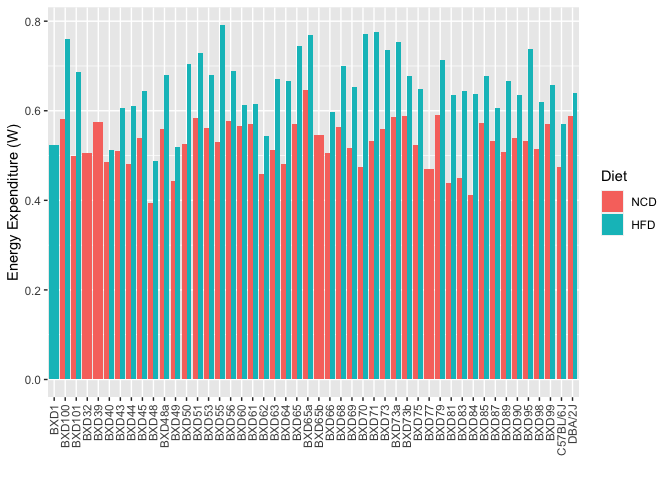
\includegraphics{figures/baseline-thermogenesis-1.png}

\begin{Shaded}
\begin{Highlighting}[]
\CommentTok{#lm(Value~Name+Diet,data=data) %>% summary}

\NormalTok{mr.order <-}\StringTok{ }
\StringTok{  }\NormalTok{data }\OperatorTok\StringTok{ }
\StringTok{  }\KeywordTok{filter}\NormalTok{(Diet }\OperatorTok{==}\StringTok{ "NCD"}\NormalTok{) }\OperatorTok\StringTok{ }
\StringTok{  }\KeywordTok{arrange}\NormalTok{(}\KeywordTok{desc}\NormalTok{(MR_W)) }\OperatorTok\StringTok{ }
\StringTok{  }\KeywordTok{mutate}\NormalTok{(}\DataTypeTok{Name =} \KeywordTok{factor}\NormalTok{(Name))}


\NormalTok{data }\OperatorTok
\StringTok{  }\KeywordTok{filter}\NormalTok{(}\OperatorTok{!}\KeywordTok{is.na}\NormalTok{(MR_W)) }\OperatorTok\StringTok{ }\CommentTok{# complete cases only}
\StringTok{  }\KeywordTok{mutate}\NormalTok{(}\DataTypeTok{Name =} \KeywordTok{factor}\NormalTok{(Name, }\DataTypeTok{levels =}\NormalTok{ mr.order}\OperatorTok{$}\NormalTok{Name, }\DataTypeTok{ordered =} \OtherTok{TRUE}\NormalTok{)) }\OperatorTok
\StringTok{  }\KeywordTok{ggplot}\NormalTok{(}\KeywordTok{aes}\NormalTok{(}\DataTypeTok{y=}\NormalTok{MR_W,}
         \DataTypeTok{x=}\NormalTok{Name,}
         \DataTypeTok{ymin=}\NormalTok{MR_W}\OperatorTok{-}\NormalTok{MR_W_SE,}
         \DataTypeTok{ymax=}\NormalTok{MR_W}\OperatorTok{+}\NormalTok{MR_W_SE,}
         \DataTypeTok{fill=}\NormalTok{Diet)) }\OperatorTok{+}
\StringTok{  }\KeywordTok{geom_bar}\NormalTok{(}\DataTypeTok{stat=}\StringTok{'identity'}\NormalTok{,}\DataTypeTok{position=}\StringTok{'dodge'}\NormalTok{, }\DataTypeTok{width=}\FloatTok{0.75}\NormalTok{) }\OperatorTok{+}
\StringTok{  }\KeywordTok{geom_errorbar}\NormalTok{(}\DataTypeTok{position=}\KeywordTok{position_dodge}\NormalTok{(}\DataTypeTok{width=}\FloatTok{0.75}\NormalTok{), }\DataTypeTok{width=}\FloatTok{0.5}\NormalTok{) }\OperatorTok{+}
\StringTok{  }\KeywordTok{labs}\NormalTok{(}\DataTypeTok{y=}\StringTok{"Energy Expenditure (W)"}\NormalTok{,}\DataTypeTok{x=}\StringTok{""}\NormalTok{) }\OperatorTok{+}
\StringTok{  }\KeywordTok{theme}\NormalTok{(}\DataTypeTok{axis.text.x =} \KeywordTok{element_text}\NormalTok{(}\DataTypeTok{angle =} \DecValTok{90}\NormalTok{, }\DataTypeTok{vjust =} \FloatTok{0.5}\NormalTok{, }\DataTypeTok{hjust=}\DecValTok{1}\NormalTok{))}
\end{Highlighting}
\end{Shaded}

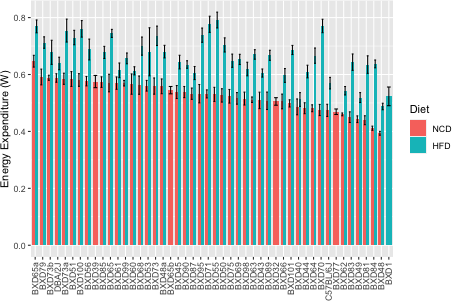
\includegraphics{figures/baseline-thermogenesis-2.png}

\hypertarget{estimating-effect-sizes}{%
\subsection{Estimating Effect Sizes}\label{estimating-effect-sizes}}

\begin{Shaded}
\begin{Highlighting}[]
\NormalTok{data }\OperatorTok
\StringTok{  }\KeywordTok{group_by}\NormalTok{(Diet) }\OperatorTok
\StringTok{  }\KeywordTok{summarize}\NormalTok{(}\DataTypeTok{Max =} \KeywordTok{max}\NormalTok{(MR_W, }\DataTypeTok{na.rm=}\NormalTok{T),}
            \DataTypeTok{Min =} \KeywordTok{min}\NormalTok{(MR_W,}\DataTypeTok{na.rm=}\NormalTok{T), }
            \DataTypeTok{Mean =} \KeywordTok{mean}\NormalTok{(MR_W, }\DataTypeTok{na.rm=}\NormalTok{T),}
            \DataTypeTok{SE =} \KeywordTok{mean}\NormalTok{(MR_W_SE,}\DataTypeTok{na.rm=}\NormalTok{T),}
            \DataTypeTok{N =} \KeywordTok{mean}\NormalTok{(N,}\DataTypeTok{na.rm=}\NormalTok{T)) }\OperatorTok
\StringTok{  }\KeywordTok{mutate}\NormalTok{(}\DataTypeTok{SD =}\NormalTok{ SE}\OperatorTok{*}\KeywordTok{sqrt}\NormalTok{(}\KeywordTok{mean}\NormalTok{(N,}\DataTypeTok{na.rm=}\NormalTok{T))) }\OperatorTok
\StringTok{  }\KeywordTok{mutate}\NormalTok{(}\DataTypeTok{Rel.SD =}\NormalTok{ SD}\OperatorTok{/}\NormalTok{Mean}\OperatorTok{*}\DecValTok{100}\NormalTok{) }\OperatorTok
\StringTok{  }\KeywordTok{kable}\NormalTok{(}\DataTypeTok{caption=}\StringTok{"Summary statistics for thermogenesis from BXD mice"}\NormalTok{)}
\end{Highlighting}
\end{Shaded}

\begin{longtable}[]{@{}lrrrrrrr@{}}
\caption{Summary statistics for thermogenesis from BXD
mice}\tabularnewline
\toprule
Diet & Max & Min & Mean & SE & N & SD & Rel.SD\tabularnewline
\midrule
\endfirsthead
\toprule
Diet & Max & Min & Mean & SE & N & SD & Rel.SD\tabularnewline
\midrule
\endhead
NCD & 0.647 & 0.393 & 0.526 & 0.020 & 4.44 & 0.042 & 7.96\tabularnewline
HFD & 0.791 & 0.488 & 0.659 & 0.025 & 4.47 & 0.052 & 7.96\tabularnewline
\bottomrule
\end{longtable}

\begin{Shaded}
\begin{Highlighting}[]
\NormalTok{data }\OperatorTok
\StringTok{  }\KeywordTok{group_by}\NormalTok{(Diet) }\OperatorTok
\StringTok{  }\KeywordTok{summarize}\NormalTok{(}\DataTypeTok{Max =} \KeywordTok{max}\NormalTok{(Value_lm, }\DataTypeTok{na.rm=}\NormalTok{T),}
            \DataTypeTok{Min =} \KeywordTok{min}\NormalTok{(Value_lm,}\DataTypeTok{na.rm=}\NormalTok{T), }
            \DataTypeTok{Mean =} \KeywordTok{mean}\NormalTok{(Value_lm, }\DataTypeTok{na.rm=}\NormalTok{T),}
            \DataTypeTok{SE =} \KeywordTok{mean}\NormalTok{(SE_lm,}\DataTypeTok{na.rm=}\NormalTok{T),}
            \DataTypeTok{N =} \KeywordTok{mean}\NormalTok{(N,}\DataTypeTok{na.rm=}\NormalTok{T)) }\OperatorTok
\StringTok{  }\KeywordTok{mutate}\NormalTok{(}\DataTypeTok{SD =}\NormalTok{ SE}\OperatorTok{*}\KeywordTok{sqrt}\NormalTok{(}\KeywordTok{mean}\NormalTok{(N,}\DataTypeTok{na.rm=}\NormalTok{T))) }\OperatorTok
\StringTok{  }\KeywordTok{mutate}\NormalTok{(}\DataTypeTok{Rel.SD =}\NormalTok{ SD}\OperatorTok{/}\NormalTok{Mean}\OperatorTok{*}\DecValTok{100}\NormalTok{) }\OperatorTok
\StringTok{  }\KeywordTok{kable}\NormalTok{(}\DataTypeTok{caption=}\StringTok{"Summary statistics for lean mass from BXD mice"}\NormalTok{)}
\end{Highlighting}
\end{Shaded}

\begin{longtable}[]{@{}lrrrrrrr@{}}
\caption{Summary statistics for lean mass from BXD mice}\tabularnewline
\toprule
Diet & Max & Min & Mean & SE & N & SD & Rel.SD\tabularnewline
\midrule
\endfirsthead
\toprule
Diet & Max & Min & Mean & SE & N & SD & Rel.SD\tabularnewline
\midrule
\endhead
NCD & 30.7 & 19.7 & 25.4 & 0.623 & 4.44 & 1.31 & 5.19\tabularnewline
HFD & 30.2 & 20.0 & 26.0 & 0.612 & 4.47 & 1.29 & 4.97\tabularnewline
\bottomrule
\end{longtable}

\hypertarget{adjusting-for-lean-mass}{%
\subsection{Adjusting for Lean Mass}\label{adjusting-for-lean-mass}}

\begin{Shaded}
\begin{Highlighting}[]
\KeywordTok{library}\NormalTok{(ggrepel)}
\KeywordTok{ggplot}\NormalTok{(data, }\KeywordTok{aes}\NormalTok{(}\DataTypeTok{y=}\NormalTok{MR_W,}
           \DataTypeTok{x=}\NormalTok{Value_lm)) }\OperatorTok{+}
\StringTok{  }\KeywordTok{geom_point}\NormalTok{(}\KeywordTok{aes}\NormalTok{(}\DataTypeTok{col=}\NormalTok{Diet)) }\OperatorTok{+}
\StringTok{  }\KeywordTok{geom_smooth}\NormalTok{(}\DataTypeTok{method=}\StringTok{"lm"}\NormalTok{) }\OperatorTok{+}
\StringTok{  }\CommentTok{#geom_label_repel(data = subset(data, (MR_W < 0.45&Value_lm>25.5)|MR_W>0.65&Value_lm<27), aes(label=Name,col=Diet)) +}
\StringTok{  }\KeywordTok{labs}\NormalTok{(}\DataTypeTok{y=}\StringTok{"Energy Expenditure (W)"}\NormalTok{,}
       \DataTypeTok{x=}\StringTok{"Lean Mass (g)"}\NormalTok{)}
\end{Highlighting}
\end{Shaded}

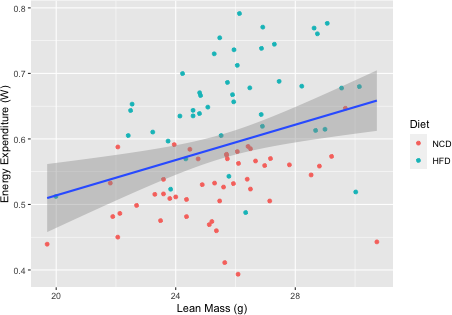
\includegraphics{figures/lean-mass-adjusting-1.png}

\begin{Shaded}
\begin{Highlighting}[]
\KeywordTok{ggplot}\NormalTok{(data, }\KeywordTok{aes}\NormalTok{(}\DataTypeTok{y=}\NormalTok{MR_W,}
           \DataTypeTok{x=}\NormalTok{Value_lm,}
           \DataTypeTok{col=}\NormalTok{Diet)) }\OperatorTok{+}
\StringTok{  }\KeywordTok{geom_point}\NormalTok{() }\OperatorTok{+}
\StringTok{  }\KeywordTok{geom_smooth}\NormalTok{(}\DataTypeTok{method=}\StringTok{"lm"}\NormalTok{) }\OperatorTok{+}
\StringTok{  }\KeywordTok{geom_errorbar}\NormalTok{(}\KeywordTok{aes}\NormalTok{(}\DataTypeTok{ymin=}\NormalTok{MR_W}\OperatorTok{-}\NormalTok{MR_W_SE,}
                \DataTypeTok{ymax=}\NormalTok{MR_W}\OperatorTok{+}\NormalTok{MR_W_SE)) }\OperatorTok{+}
\StringTok{  }\KeywordTok{geom_errorbarh}\NormalTok{(}\KeywordTok{aes}\NormalTok{(}\DataTypeTok{xmin=}\NormalTok{Value_lm}\OperatorTok{-}\NormalTok{SE_lm,}
                \DataTypeTok{xmax=}\NormalTok{Value_lm}\OperatorTok{+}\NormalTok{SE_lm))}\OperatorTok{+}
\StringTok{  }\CommentTok{#geom_label_repel(data = subset(data, (MR_W < 0.45&Value_lm>25.5)|MR_W>0.65&Value_lm<27),aes(label=Name)) +}
\StringTok{  }\KeywordTok{labs}\NormalTok{(}\DataTypeTok{y=}\StringTok{"Energy Expenditure (W)"}\NormalTok{,}
       \DataTypeTok{x=}\StringTok{"Lean Mass (g)"}\NormalTok{) }\OperatorTok{+}
\StringTok{  }\KeywordTok{theme_classic}\NormalTok{() }\OperatorTok{+}
\StringTok{  }\KeywordTok{theme}\NormalTok{(}\DataTypeTok{legend.position =} \KeywordTok{c}\NormalTok{(}\FloatTok{0.1}\NormalTok{,}\FloatTok{0.85}\NormalTok{),}
        \DataTypeTok{text=}\KeywordTok{element_text}\NormalTok{(}\DataTypeTok{size=}\DecValTok{18}\NormalTok{))}
\end{Highlighting}
\end{Shaded}

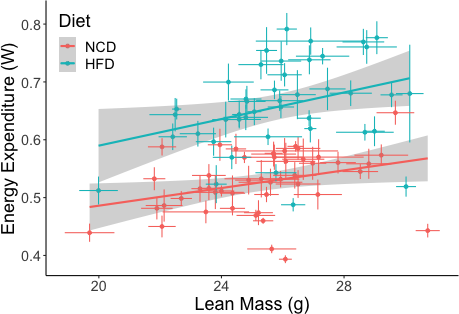
\includegraphics{figures/lean-mass-adjusting-2.png}

\begin{Shaded}
\begin{Highlighting}[]
\CommentTok{#chow only}
\KeywordTok{ggplot}\NormalTok{(data }\OperatorTok\StringTok{ }\KeywordTok{filter}\NormalTok{(Diet}\OperatorTok{==}\StringTok{"NCD"}\NormalTok{), }\KeywordTok{aes}\NormalTok{(}\DataTypeTok{y=}\NormalTok{MR_W,}
           \DataTypeTok{x=}\NormalTok{Value_lm)) }\OperatorTok{+}
\StringTok{  }\KeywordTok{geom_point}\NormalTok{() }\OperatorTok{+}
\StringTok{  }\KeywordTok{geom_smooth}\NormalTok{(}\DataTypeTok{method=}\StringTok{"lm"}\NormalTok{) }\OperatorTok{+}
\StringTok{  }\KeywordTok{geom_label_repel}\NormalTok{(}\DataTypeTok{data =} \KeywordTok{subset}\NormalTok{(data }\OperatorTok\StringTok{ }\KeywordTok{filter}\NormalTok{(Diet}\OperatorTok{==}\StringTok{"NCD"}\NormalTok{),}
\NormalTok{                                 (MR_W }\OperatorTok{<}\StringTok{ }\FloatTok{0.43}\OperatorTok{&}\NormalTok{Value_lm}\OperatorTok{>}\FloatTok{24.5}\NormalTok{)}\OperatorTok{|}\NormalTok{MR_W}\OperatorTok{>}\FloatTok{0.60}\OperatorTok{&}\NormalTok{Value_lm}\OperatorTok{<}\DecValTok{27}\NormalTok{),}
                   \KeywordTok{aes}\NormalTok{(}\DataTypeTok{label=}\NormalTok{Name)) }\OperatorTok{+}
\StringTok{  }\KeywordTok{guides}\NormalTok{(}\DataTypeTok{fill =} \KeywordTok{guide_legend}\NormalTok{(}\DataTypeTok{override.aes =} \KeywordTok{aes}\NormalTok{(}\DataTypeTok{color =} \OtherTok{NA}\NormalTok{))) }\OperatorTok{+}
\StringTok{  }\KeywordTok{labs}\NormalTok{(}\DataTypeTok{y=}\StringTok{"Energy Expenditure (W)"}\NormalTok{,}
       \DataTypeTok{x=}\StringTok{"Lean Mass (g)"}\NormalTok{)}
\end{Highlighting}
\end{Shaded}

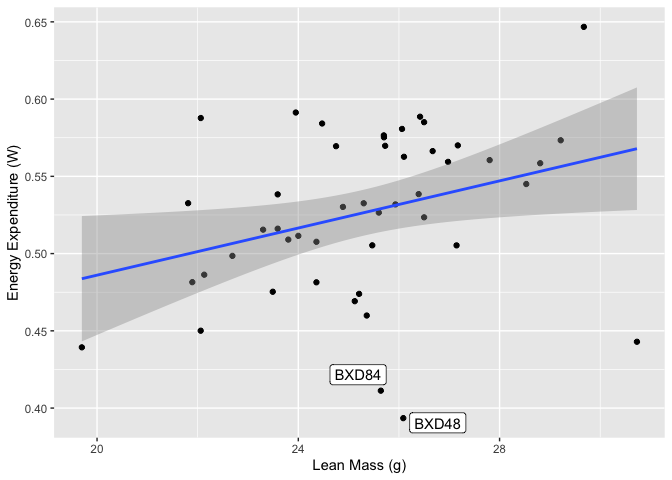
\includegraphics{figures/lean-mass-adjusting-3.png}

\begin{Shaded}
\begin{Highlighting}[]
\NormalTok{lm.model}\FloatTok{.1}\NormalTok{ <-}\StringTok{ }\KeywordTok{lm}\NormalTok{(MR_W}\OperatorTok{~}\NormalTok{Value_lm,}\DataTypeTok{data=}\NormalTok{data }\OperatorTok\StringTok{ }\KeywordTok{filter}\NormalTok{(Diet}\OperatorTok{==}\StringTok{"NCD"}\NormalTok{)) }\CommentTok{#model built on only NCD}
\NormalTok{lm.model}\FloatTok{.2}\NormalTok{ <-}\StringTok{ }\KeywordTok{lm}\NormalTok{(MR_W}\OperatorTok{~}\NormalTok{Value_lm}\OperatorTok{+}\NormalTok{Diet,}\DataTypeTok{data=}\NormalTok{data) }\CommentTok{#model built on NCD and AT}
\KeywordTok{library}\NormalTok{(broom)}
\KeywordTok{aov}\NormalTok{(lm.model}\FloatTok{.1}\NormalTok{) }\OperatorTok\StringTok{ }\NormalTok{tidy }\OperatorTok\StringTok{ }\KeywordTok{kable}\NormalTok{(}\DataTypeTok{caption=}\StringTok{"Model 1 summary for adjusting for lean mass"}\NormalTok{)}
\end{Highlighting}
\end{Shaded}

\begin{longtable}[]{@{}lrrrrr@{}}
\caption{Model 1 summary for adjusting for lean mass}\tabularnewline
\toprule
term & df & sumsq & meansq & statistic & p.value\tabularnewline
\midrule
\endfirsthead
\toprule
term & df & sumsq & meansq & statistic & p.value\tabularnewline
\midrule
\endhead
Value\_lm & 1 & 0.013 & 0.013 & 5.17 & 0.028\tabularnewline
Residuals & 45 & 0.115 & 0.003 & NA & NA\tabularnewline
\bottomrule
\end{longtable}

\begin{Shaded}
\begin{Highlighting}[]
\KeywordTok{summary}\NormalTok{(lm.model}\FloatTok{.1}\NormalTok{) }\OperatorTok\StringTok{ }\NormalTok{tidy }\OperatorTok\StringTok{ }\KeywordTok{kable}\NormalTok{(}\DataTypeTok{caption=}\StringTok{"Model 1 coefficients for adjusting for lean mass"}\NormalTok{)}
\end{Highlighting}
\end{Shaded}

\begin{longtable}[]{@{}lrrrr@{}}
\caption{Model 1 coefficients for adjusting for lean
mass}\tabularnewline
\toprule
term & estimate & std.error & statistic & p.value\tabularnewline
\midrule
\endfirsthead
\toprule
term & estimate & std.error & statistic & p.value\tabularnewline
\midrule
\endhead
(Intercept) & 0.333 & 0.085 & 3.92 & 0.000\tabularnewline
Value\_lm & 0.008 & 0.003 & 2.27 & 0.028\tabularnewline
\bottomrule
\end{longtable}

\begin{Shaded}
\begin{Highlighting}[]
\KeywordTok{aov}\NormalTok{(lm.model}\FloatTok{.2}\NormalTok{) }\OperatorTok\StringTok{ }\NormalTok{tidy }\OperatorTok\StringTok{ }\KeywordTok{kable}\NormalTok{(}\DataTypeTok{caption=}\StringTok{"Model 2 summary for adjusting for lean mass"}\NormalTok{)}
\end{Highlighting}
\end{Shaded}

\begin{longtable}[]{@{}lrrrrr@{}}
\caption{Model 2 summary for adjusting for lean mass}\tabularnewline
\toprule
term & df & sumsq & meansq & statistic & p.value\tabularnewline
\midrule
\endfirsthead
\toprule
term & df & sumsq & meansq & statistic & p.value\tabularnewline
\midrule
\endhead
Value\_lm & 1 & 0.081 & 0.081 & 21.5 & 0\tabularnewline
Diet & 1 & 0.347 & 0.347 & 92.0 & 0\tabularnewline
Residuals & 87 & 0.328 & 0.004 & NA & NA\tabularnewline
\bottomrule
\end{longtable}

\begin{Shaded}
\begin{Highlighting}[]
\KeywordTok{summary}\NormalTok{(lm.model}\FloatTok{.2}\NormalTok{) }\OperatorTok\StringTok{ }\NormalTok{tidy }\OperatorTok\StringTok{ }\KeywordTok{kable}\NormalTok{(}\DataTypeTok{caption=}\StringTok{"Model 2 coefficients for adjusting for lean mass"}\NormalTok{)}
\end{Highlighting}
\end{Shaded}

\begin{longtable}[]{@{}lrrrr@{}}
\caption{Model 2 coefficients for adjusting for lean
mass}\tabularnewline
\toprule
term & estimate & std.error & statistic & p.value\tabularnewline
\midrule
\endfirsthead
\toprule
term & estimate & std.error & statistic & p.value\tabularnewline
\midrule
\endhead
(Intercept) & 0.287 & 0.075 & 3.83 & 0.000\tabularnewline
Value\_lm & 0.009 & 0.003 & 3.22 & 0.002\tabularnewline
DietHFD & 0.126 & 0.013 & 9.59 & 0.000\tabularnewline
\bottomrule
\end{longtable}

\begin{Shaded}
\begin{Highlighting}[]
\NormalTok{data <-}\StringTok{ }\NormalTok{data }\OperatorTok
\StringTok{  }\KeywordTok{mutate}\NormalTok{(}\DataTypeTok{MR_predicted =} \KeywordTok{predict}\NormalTok{(lm.model}\FloatTok{.1}\NormalTok{, }\DataTypeTok{newdata =} \KeywordTok{list}\NormalTok{(}\DataTypeTok{Value_lm=}\NormalTok{Value_lm))) }\OperatorTok
\StringTok{  }\KeywordTok{mutate}\NormalTok{(}\DataTypeTok{MR_resid =}\NormalTok{ MR_W}\OperatorTok{-}\NormalTok{MR_predicted) }\OperatorTok
\StringTok{  }\KeywordTok{mutate}\NormalTok{(}\DataTypeTok{MR_adj =}\NormalTok{ MR_resid }\OperatorTok{+}\StringTok{ }\KeywordTok{coef}\NormalTok{(lm.model}\FloatTok{.1}\NormalTok{)[}\StringTok{'(Intercept)'}\NormalTok{] }\OperatorTok{+}\StringTok{ }\KeywordTok{coef}\NormalTok{(lm.model}\FloatTok{.2}\NormalTok{)[}\StringTok{'Value_lm'}\NormalTok{]}\OperatorTok{*}\KeywordTok{mean}\NormalTok{(data}\OperatorTok{$}\NormalTok{Value_lm,}\DataTypeTok{na.rm=}\NormalTok{T))}

\NormalTok{data }\OperatorTok
\StringTok{  }\KeywordTok{filter}\NormalTok{(}\OperatorTok{!}\KeywordTok{is.na}\NormalTok{(MR_W)) }\OperatorTok\StringTok{ }\CommentTok{# complete cases only}
\StringTok{  }\KeywordTok{ggplot}\NormalTok{(}\KeywordTok{aes}\NormalTok{(}\DataTypeTok{y=}\NormalTok{MR_resid,}
         \DataTypeTok{x=}\KeywordTok{reorder}\NormalTok{(Name,}\OperatorTok{-}\NormalTok{MR_W),}
         \DataTypeTok{ymin=}\NormalTok{MR_resid}\OperatorTok{-}\NormalTok{MR_W_SE,}
         \DataTypeTok{ymax=}\NormalTok{MR_resid}\OperatorTok{-}\NormalTok{MR_W_SE,}
         \DataTypeTok{fill=}\NormalTok{Diet)) }\OperatorTok{+}
\StringTok{  }\CommentTok{#geom_label_repel(label=Name) +}
\StringTok{  }\KeywordTok{geom_bar}\NormalTok{(}\DataTypeTok{stat=}\StringTok{'identity'}\NormalTok{,}\DataTypeTok{position=}\StringTok{'dodge'}\NormalTok{) }\OperatorTok{+}
\StringTok{  }\KeywordTok{labs}\NormalTok{(}\DataTypeTok{y=}\StringTok{"EE Observed - EE Predicted (W)"}\NormalTok{) }\OperatorTok{+}
\StringTok{  }\KeywordTok{theme}\NormalTok{(}\DataTypeTok{axis.text.x =} \KeywordTok{element_text}\NormalTok{(}\DataTypeTok{angle =} \DecValTok{90}\NormalTok{, }\DataTypeTok{vjust =} \FloatTok{0.5}\NormalTok{, }\DataTypeTok{hjust=}\DecValTok{1}\NormalTok{))}
\end{Highlighting}
\end{Shaded}

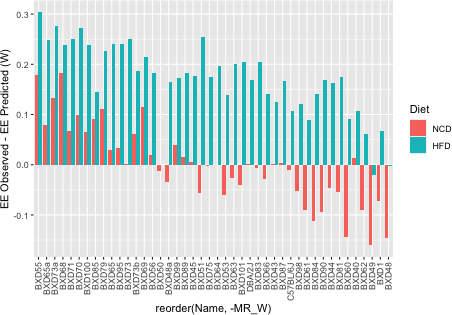
\includegraphics{figures/lean-mass-adjusting-4.png}

\begin{Shaded}
\begin{Highlighting}[]
\NormalTok{mr.adj.order <-}\StringTok{ }
\StringTok{  }\NormalTok{data }\OperatorTok\StringTok{ }
\StringTok{  }\KeywordTok{filter}\NormalTok{(Diet }\OperatorTok{==}\StringTok{ "NCD"}\NormalTok{) }\OperatorTok\StringTok{ }
\StringTok{  }\KeywordTok{arrange}\NormalTok{(}\KeywordTok{desc}\NormalTok{(MR_adj)) }\OperatorTok\StringTok{ }
\StringTok{  }\KeywordTok{mutate}\NormalTok{(}\DataTypeTok{Name =} \KeywordTok{factor}\NormalTok{(Name))}


\NormalTok{data }\OperatorTok
\StringTok{  }\KeywordTok{filter}\NormalTok{(}\OperatorTok{!}\KeywordTok{is.na}\NormalTok{(MR_W)) }\OperatorTok\StringTok{ }\CommentTok{# complete cases only}
\StringTok{  }\KeywordTok{mutate}\NormalTok{(}\DataTypeTok{Name =} \KeywordTok{factor}\NormalTok{(Name, }\DataTypeTok{levels =}\NormalTok{ mr.adj.order}\OperatorTok{$}\NormalTok{Name, }\DataTypeTok{ordered =} \OtherTok{TRUE}\NormalTok{)) }\OperatorTok
\StringTok{  }\KeywordTok{ggplot}\NormalTok{(}\KeywordTok{aes}\NormalTok{(}\DataTypeTok{y=}\NormalTok{MR_adj,}
         \DataTypeTok{x=}\NormalTok{Name,}
         \DataTypeTok{ymin=}\NormalTok{MR_adj}\OperatorTok{-}\NormalTok{MR_W_SE,}
         \DataTypeTok{ymax=}\NormalTok{MR_adj}\OperatorTok{+}\NormalTok{MR_W_SE,}
         \DataTypeTok{fill=}\NormalTok{Diet)) }\OperatorTok{+}
\StringTok{  }\KeywordTok{geom_bar}\NormalTok{(}\DataTypeTok{stat=}\StringTok{'identity'}\NormalTok{,}\DataTypeTok{position=}\StringTok{'dodge'}\NormalTok{, }\DataTypeTok{width=}\FloatTok{0.75}\NormalTok{) }\OperatorTok{+}
\StringTok{  }\KeywordTok{geom_errorbar}\NormalTok{(}\DataTypeTok{position=}\KeywordTok{position_dodge}\NormalTok{(}\DataTypeTok{width=}\FloatTok{0.75}\NormalTok{), }\DataTypeTok{width=}\FloatTok{0.5}\NormalTok{) }\OperatorTok{+}
\StringTok{  }\KeywordTok{labs}\NormalTok{(}\DataTypeTok{y=}\StringTok{"Lean Mass Adjusted Energy Expenditure (W)"}\NormalTok{,}\DataTypeTok{x=}\StringTok{""}\NormalTok{) }\OperatorTok{+}
\StringTok{  }\KeywordTok{theme}\NormalTok{(}\DataTypeTok{axis.text.x =} \KeywordTok{element_text}\NormalTok{(}\DataTypeTok{angle =} \DecValTok{90}\NormalTok{, }\DataTypeTok{vjust =} \FloatTok{0.5}\NormalTok{, }\DataTypeTok{hjust=}\DecValTok{1}\NormalTok{))}
\end{Highlighting}
\end{Shaded}

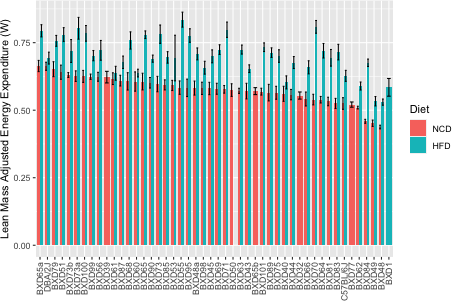
\includegraphics{figures/lean-mass-adjusting-5.png}

based on this modelling after adjusting for lean mass, HFD increases
thermogenesis by
\texttt{(coef(lm.model.2){[}"(Intercept)"{]}-coef(lm.model.2){[}"DietHFD"{]})/coef(lm.model.2){[}"(Intercept)"{]}*100}\%.

\hypertarget{adaptive-thermogenesis}{%
\subsection{Adaptive Thermogenesis}\label{adaptive-thermogenesis}}

Defined as lean mass adjusted VO2 from HFD - NCD

\begin{Shaded}
\begin{Highlighting}[]
\NormalTok{data.wide <-}
\StringTok{  }\NormalTok{data }\OperatorTok
\StringTok{  }\KeywordTok{select}\NormalTok{(Value_lm,SE,Value_bw, MR_W, MR_W_SE, MR_adj,Name,Diet) }\OperatorTok
\StringTok{  }\KeywordTok{pivot_wider}\NormalTok{(}\DataTypeTok{names_from=}\NormalTok{Diet,}\DataTypeTok{id_cols=}\NormalTok{Name,}\DataTypeTok{values_from=}\KeywordTok{c}\NormalTok{(Value_lm,Value_bw, MR_W,MR_W_SE,MR_adj,SE)) }\OperatorTok
\StringTok{  }\KeywordTok{mutate}\NormalTok{(}\DataTypeTok{AT =}\NormalTok{ MR_W_HFD }\OperatorTok{-}\StringTok{ }\NormalTok{MR_W_NCD,}
         \DataTypeTok{AT_SE =} \KeywordTok{sqrt}\NormalTok{((MR_W_SE_NCD}\OperatorTok{/}\NormalTok{MR_W_NCD)}\OperatorTok{^}\DecValTok{2}\OperatorTok{+}\NormalTok{(MR_W_SE_HFD}\OperatorTok{/}\NormalTok{MR_W_HFD)}\OperatorTok{^}\DecValTok{2}\NormalTok{)}\OperatorTok{*}\NormalTok{AT,}
         \DataTypeTok{Wt_SE =} \KeywordTok{sqrt}\NormalTok{((SE_NCD}\OperatorTok{/}\NormalTok{Value_bw_NCD)}\OperatorTok{^}\DecValTok{2}\OperatorTok{+}\NormalTok{(SE_HFD}\OperatorTok{/}\NormalTok{Value_bw_NCD)}\OperatorTok{^}\DecValTok{2}\NormalTok{)}\OperatorTok{*}\NormalTok{Value_bw_NCD,}
         \DataTypeTok{Wt.Gain =}\NormalTok{ Value_bw_HFD}\OperatorTok{-}\NormalTok{Value_bw_NCD)}

\NormalTok{data.wide }\OperatorTok
\StringTok{  }\KeywordTok{filter}\NormalTok{(}\OperatorTok{!}\KeywordTok{is.na}\NormalTok{(AT)) }\OperatorTok\StringTok{ }\CommentTok{# complete cases only}
\StringTok{  }\KeywordTok{ggplot}\NormalTok{(}\KeywordTok{aes}\NormalTok{(}\DataTypeTok{y=}\NormalTok{AT,}
         \DataTypeTok{x=}\KeywordTok{reorder}\NormalTok{(Name,}\OperatorTok{-}\NormalTok{AT),}
         \DataTypeTok{ymin=}\NormalTok{AT}\OperatorTok{-}\NormalTok{AT_SE,}
         \DataTypeTok{ymax=}\NormalTok{AT}\OperatorTok{+}\NormalTok{AT_SE)) }\OperatorTok{+}
\StringTok{  }\KeywordTok{geom_bar}\NormalTok{(}\DataTypeTok{stat=}\StringTok{'identity'}\NormalTok{,}\DataTypeTok{position=}\StringTok{'dodge'}\NormalTok{) }\OperatorTok{+}
\StringTok{    }\KeywordTok{geom_errorbar}\NormalTok{() }\OperatorTok{+}
\StringTok{  }\KeywordTok{labs}\NormalTok{(}\DataTypeTok{y=}\StringTok{"HFD-Induced Adaptive Thermogenesis (W)"}\NormalTok{,}
       \DataTypeTok{x=}\StringTok{""}\NormalTok{) }\OperatorTok{+}
\StringTok{  }\KeywordTok{theme}\NormalTok{(}\DataTypeTok{axis.text.x =} \KeywordTok{element_text}\NormalTok{(}\DataTypeTok{angle =} \DecValTok{90}\NormalTok{, }\DataTypeTok{vjust =} \FloatTok{0.5}\NormalTok{, }\DataTypeTok{hjust=}\DecValTok{1}\NormalTok{))  }
\end{Highlighting}
\end{Shaded}

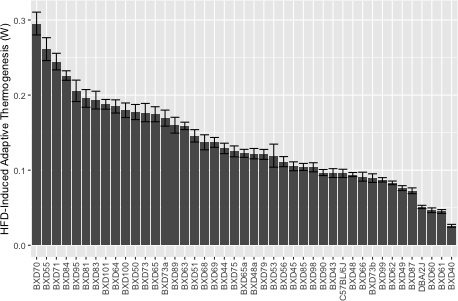
\includegraphics{figures/adaptive-thermogenesis-1.png}

\hypertarget{thermogenesis-on-ncd-as-a-predictor-of-weight-gain}{%
\subsubsection{Thermogenesis on NCD as a Predictor of Weight
Gain}\label{thermogenesis-on-ncd-as-a-predictor-of-weight-gain}}

\begin{Shaded}
\begin{Highlighting}[]
\NormalTok{data.wide }\OperatorTok
\StringTok{  }\KeywordTok{ggplot}\NormalTok{(}\KeywordTok{aes}\NormalTok{(}\DataTypeTok{y=}\NormalTok{Wt.Gain,}
             \DataTypeTok{x=}\NormalTok{MR_W_NCD)) }\OperatorTok{+}
\StringTok{  }\KeywordTok{labs}\NormalTok{(}\DataTypeTok{y=}\StringTok{"Weight Gained on HFD (g)"}\NormalTok{,}
       \DataTypeTok{x=}\StringTok{"Energy Expenditure on NCD (W)"}\NormalTok{) }\OperatorTok{+}
\StringTok{  }\KeywordTok{geom_point}\NormalTok{() }\OperatorTok{+}
\StringTok{  }\KeywordTok{geom_smooth}\NormalTok{(}\DataTypeTok{method=}\StringTok{"lm"}\NormalTok{) }\OperatorTok{+}
\StringTok{  }\KeywordTok{theme_classic}\NormalTok{() }\OperatorTok{+}
\StringTok{  }\KeywordTok{theme}\NormalTok{(}\DataTypeTok{text=}\KeywordTok{element_text}\NormalTok{(}\DataTypeTok{size=}\DecValTok{18}\NormalTok{))}
\end{Highlighting}
\end{Shaded}

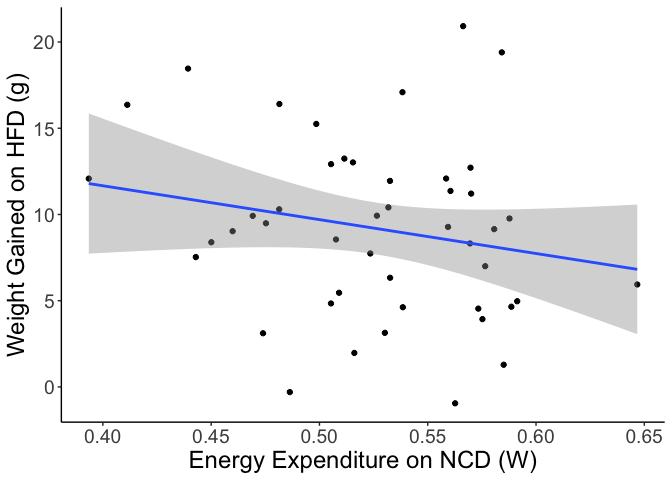
\includegraphics{figures/thermogenesis-weight-1.png}

\begin{Shaded}
\begin{Highlighting}[]
\KeywordTok{lm}\NormalTok{(Wt.Gain}\OperatorTok{~}\NormalTok{MR_W_NCD, }\DataTypeTok{data=}\NormalTok{data.wide) }\OperatorTok\StringTok{ }\NormalTok{glance }\OperatorTok\StringTok{ }\KeywordTok{kable}\NormalTok{(}\DataTypeTok{caption=}\StringTok{"Summary of relationship between energy expenditure and diet-induced weight gain"}\NormalTok{, }\DataTypeTok{digits =} \KeywordTok{c}\NormalTok{(}\DecValTok{3}\NormalTok{,}\DecValTok{3}\NormalTok{,}\DecValTok{3}\NormalTok{,}\DecValTok{1}\NormalTok{,}\DecValTok{8}\NormalTok{,}\DecValTok{0}\NormalTok{,}\DecValTok{0}\NormalTok{,}\DecValTok{0}\NormalTok{,}\DecValTok{0}\NormalTok{,}\DecValTok{0}\NormalTok{,}\DecValTok{0}\NormalTok{,}\DecValTok{0}\NormalTok{))}
\end{Highlighting}
\end{Shaded}

\begin{longtable}[]{@{}rrrrrrrrrrrr@{}}
\caption{Summary of relationship between energy expenditure and
diet-induced weight gain}\tabularnewline
\toprule
\begin{minipage}[b]{0.08\columnwidth}\raggedleft
r.squared\strut
\end{minipage} & \begin{minipage}[b]{0.11\columnwidth}\raggedleft
adj.r.squared\strut
\end{minipage} & \begin{minipage}[b]{0.05\columnwidth}\raggedleft
sigma\strut
\end{minipage} & \begin{minipage}[b]{0.08\columnwidth}\raggedleft
statistic\strut
\end{minipage} & \begin{minipage}[b]{0.06\columnwidth}\raggedleft
p.value\strut
\end{minipage} & \begin{minipage}[b]{0.02\columnwidth}\raggedleft
df\strut
\end{minipage} & \begin{minipage}[b]{0.05\columnwidth}\raggedleft
logLik\strut
\end{minipage} & \begin{minipage}[b]{0.03\columnwidth}\raggedleft
AIC\strut
\end{minipage} & \begin{minipage}[b]{0.03\columnwidth}\raggedleft
BIC\strut
\end{minipage} & \begin{minipage}[b]{0.07\columnwidth}\raggedleft
deviance\strut
\end{minipage} & \begin{minipage}[b]{0.09\columnwidth}\raggedleft
df.residual\strut
\end{minipage} & \begin{minipage}[b]{0.04\columnwidth}\raggedleft
nobs\strut
\end{minipage}\tabularnewline
\midrule
\endfirsthead
\toprule
\begin{minipage}[b]{0.08\columnwidth}\raggedleft
r.squared\strut
\end{minipage} & \begin{minipage}[b]{0.11\columnwidth}\raggedleft
adj.r.squared\strut
\end{minipage} & \begin{minipage}[b]{0.05\columnwidth}\raggedleft
sigma\strut
\end{minipage} & \begin{minipage}[b]{0.08\columnwidth}\raggedleft
statistic\strut
\end{minipage} & \begin{minipage}[b]{0.06\columnwidth}\raggedleft
p.value\strut
\end{minipage} & \begin{minipage}[b]{0.02\columnwidth}\raggedleft
df\strut
\end{minipage} & \begin{minipage}[b]{0.05\columnwidth}\raggedleft
logLik\strut
\end{minipage} & \begin{minipage}[b]{0.03\columnwidth}\raggedleft
AIC\strut
\end{minipage} & \begin{minipage}[b]{0.03\columnwidth}\raggedleft
BIC\strut
\end{minipage} & \begin{minipage}[b]{0.07\columnwidth}\raggedleft
deviance\strut
\end{minipage} & \begin{minipage}[b]{0.09\columnwidth}\raggedleft
df.residual\strut
\end{minipage} & \begin{minipage}[b]{0.04\columnwidth}\raggedleft
nobs\strut
\end{minipage}\tabularnewline
\midrule
\endhead
\begin{minipage}[t]{0.08\columnwidth}\raggedleft
0.042\strut
\end{minipage} & \begin{minipage}[t]{0.11\columnwidth}\raggedleft
0.02\strut
\end{minipage} & \begin{minipage}[t]{0.05\columnwidth}\raggedleft
5.06\strut
\end{minipage} & \begin{minipage}[t]{0.08\columnwidth}\raggedleft
1.9\strut
\end{minipage} & \begin{minipage}[t]{0.06\columnwidth}\raggedleft
0.172\strut
\end{minipage} & \begin{minipage}[t]{0.02\columnwidth}\raggedleft
1\strut
\end{minipage} & \begin{minipage}[t]{0.05\columnwidth}\raggedleft
-139\strut
\end{minipage} & \begin{minipage}[t]{0.03\columnwidth}\raggedleft
284\strut
\end{minipage} & \begin{minipage}[t]{0.03\columnwidth}\raggedleft
289\strut
\end{minipage} & \begin{minipage}[t]{0.07\columnwidth}\raggedleft
1128\strut
\end{minipage} & \begin{minipage}[t]{0.09\columnwidth}\raggedleft
44\strut
\end{minipage} & \begin{minipage}[t]{0.04\columnwidth}\raggedleft
46\strut
\end{minipage}\tabularnewline
\bottomrule
\end{longtable}

\begin{Shaded}
\begin{Highlighting}[]
\NormalTok{data.wide }\OperatorTok
\StringTok{  }\KeywordTok{ggplot}\NormalTok{(}\KeywordTok{aes}\NormalTok{(}\DataTypeTok{y=}\NormalTok{Wt.Gain,}
             \DataTypeTok{x=}\NormalTok{MR_adj_NCD)) }\OperatorTok{+}
\StringTok{  }\KeywordTok{labs}\NormalTok{(}\DataTypeTok{y=}\StringTok{"Weight Gained on HFD (g)"}\NormalTok{,}
       \DataTypeTok{x=}\StringTok{"Adjusted Energy Expenditure on NCD (W)"}\NormalTok{) }\OperatorTok{+}
\StringTok{  }\KeywordTok{geom_point}\NormalTok{() }\OperatorTok{+}
\StringTok{  }\KeywordTok{geom_smooth}\NormalTok{(}\DataTypeTok{method=}\StringTok{"lm"}\NormalTok{) }\OperatorTok{+}
\StringTok{  }\KeywordTok{geom_errorbarh}\NormalTok{(}\KeywordTok{aes}\NormalTok{(}\DataTypeTok{xmin=}\NormalTok{MR_adj_NCD}\OperatorTok{-}\NormalTok{MR_W_SE_NCD,}
                    \DataTypeTok{xmax=}\NormalTok{MR_adj_NCD}\OperatorTok{+}\NormalTok{MR_W_SE_NCD))}\OperatorTok{+}
\StringTok{  }\KeywordTok{geom_errorbar}\NormalTok{(}\KeywordTok{aes}\NormalTok{(}\DataTypeTok{ymin=}\NormalTok{Wt.Gain}\OperatorTok{-}\NormalTok{Wt_SE,}
                     \DataTypeTok{ymax=}\NormalTok{Wt.Gain}\OperatorTok{+}\NormalTok{Wt_SE)) }\OperatorTok{+}
\StringTok{  }\KeywordTok{theme_classic}\NormalTok{() }\OperatorTok{+}
\StringTok{  }\KeywordTok{theme}\NormalTok{(}\DataTypeTok{text=}\KeywordTok{element_text}\NormalTok{(}\DataTypeTok{size=}\DecValTok{18}\NormalTok{))}
\end{Highlighting}
\end{Shaded}

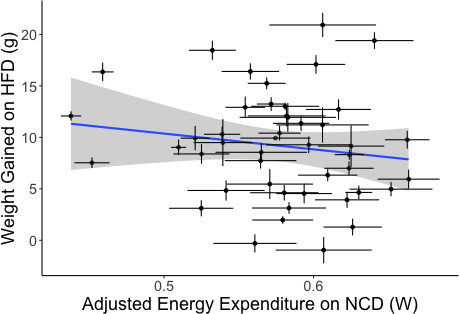
\includegraphics{figures/thermogenesis-weight-2.png}

\begin{Shaded}
\begin{Highlighting}[]
\KeywordTok{lm}\NormalTok{(Wt.Gain}\OperatorTok{~}\NormalTok{MR_adj_NCD, }\DataTypeTok{data=}\NormalTok{data.wide) }\OperatorTok\StringTok{ }\NormalTok{glance }\OperatorTok\StringTok{ }\KeywordTok{kable}\NormalTok{(}\DataTypeTok{caption=}\StringTok{"Summary of relationship between lean mass adjusted energy expenditure and diet-induced weight gain"}\NormalTok{, }\DataTypeTok{digits =} \KeywordTok{c}\NormalTok{(}\DecValTok{3}\NormalTok{,}\DecValTok{3}\NormalTok{,}\DecValTok{3}\NormalTok{,}\DecValTok{1}\NormalTok{,}\DecValTok{8}\NormalTok{,}\DecValTok{0}\NormalTok{,}\DecValTok{0}\NormalTok{,}\DecValTok{0}\NormalTok{,}\DecValTok{0}\NormalTok{,}\DecValTok{0}\NormalTok{,}\DecValTok{0}\NormalTok{,}\DecValTok{0}\NormalTok{))}
\end{Highlighting}
\end{Shaded}

\begin{longtable}[]{@{}rrrrrrrrrrrr@{}}
\caption{Summary of relationship between lean mass adjusted energy
expenditure and diet-induced weight gain}\tabularnewline
\toprule
\begin{minipage}[b]{0.08\columnwidth}\raggedleft
r.squared\strut
\end{minipage} & \begin{minipage}[b]{0.11\columnwidth}\raggedleft
adj.r.squared\strut
\end{minipage} & \begin{minipage}[b]{0.05\columnwidth}\raggedleft
sigma\strut
\end{minipage} & \begin{minipage}[b]{0.08\columnwidth}\raggedleft
statistic\strut
\end{minipage} & \begin{minipage}[b]{0.06\columnwidth}\raggedleft
p.value\strut
\end{minipage} & \begin{minipage}[b]{0.02\columnwidth}\raggedleft
df\strut
\end{minipage} & \begin{minipage}[b]{0.05\columnwidth}\raggedleft
logLik\strut
\end{minipage} & \begin{minipage}[b]{0.03\columnwidth}\raggedleft
AIC\strut
\end{minipage} & \begin{minipage}[b]{0.03\columnwidth}\raggedleft
BIC\strut
\end{minipage} & \begin{minipage}[b]{0.07\columnwidth}\raggedleft
deviance\strut
\end{minipage} & \begin{minipage}[b]{0.09\columnwidth}\raggedleft
df.residual\strut
\end{minipage} & \begin{minipage}[b]{0.04\columnwidth}\raggedleft
nobs\strut
\end{minipage}\tabularnewline
\midrule
\endfirsthead
\toprule
\begin{minipage}[b]{0.08\columnwidth}\raggedleft
r.squared\strut
\end{minipage} & \begin{minipage}[b]{0.11\columnwidth}\raggedleft
adj.r.squared\strut
\end{minipage} & \begin{minipage}[b]{0.05\columnwidth}\raggedleft
sigma\strut
\end{minipage} & \begin{minipage}[b]{0.08\columnwidth}\raggedleft
statistic\strut
\end{minipage} & \begin{minipage}[b]{0.06\columnwidth}\raggedleft
p.value\strut
\end{minipage} & \begin{minipage}[b]{0.02\columnwidth}\raggedleft
df\strut
\end{minipage} & \begin{minipage}[b]{0.05\columnwidth}\raggedleft
logLik\strut
\end{minipage} & \begin{minipage}[b]{0.03\columnwidth}\raggedleft
AIC\strut
\end{minipage} & \begin{minipage}[b]{0.03\columnwidth}\raggedleft
BIC\strut
\end{minipage} & \begin{minipage}[b]{0.07\columnwidth}\raggedleft
deviance\strut
\end{minipage} & \begin{minipage}[b]{0.09\columnwidth}\raggedleft
df.residual\strut
\end{minipage} & \begin{minipage}[b]{0.04\columnwidth}\raggedleft
nobs\strut
\end{minipage}\tabularnewline
\midrule
\endhead
\begin{minipage}[t]{0.08\columnwidth}\raggedleft
0.023\strut
\end{minipage} & \begin{minipage}[t]{0.11\columnwidth}\raggedleft
0.001\strut
\end{minipage} & \begin{minipage}[t]{0.05\columnwidth}\raggedleft
5.11\strut
\end{minipage} & \begin{minipage}[t]{0.08\columnwidth}\raggedleft
1\strut
\end{minipage} & \begin{minipage}[t]{0.06\columnwidth}\raggedleft
0.315\strut
\end{minipage} & \begin{minipage}[t]{0.02\columnwidth}\raggedleft
1\strut
\end{minipage} & \begin{minipage}[t]{0.05\columnwidth}\raggedleft
-139\strut
\end{minipage} & \begin{minipage}[t]{0.03\columnwidth}\raggedleft
285\strut
\end{minipage} & \begin{minipage}[t]{0.03\columnwidth}\raggedleft
290\strut
\end{minipage} & \begin{minipage}[t]{0.07\columnwidth}\raggedleft
1151\strut
\end{minipage} & \begin{minipage}[t]{0.09\columnwidth}\raggedleft
44\strut
\end{minipage} & \begin{minipage}[t]{0.04\columnwidth}\raggedleft
46\strut
\end{minipage}\tabularnewline
\bottomrule
\end{longtable}

\begin{Shaded}
\begin{Highlighting}[]
\NormalTok{gemma.phenotype.export <-}\StringTok{ 'Strain Level Energy Expenditure Data.csv'}
\NormalTok{data }\OperatorTok
\StringTok{  }\KeywordTok{filter}\NormalTok{(Diet}\OperatorTok{==}\StringTok{"NCD"}\NormalTok{) }\OperatorTok
\StringTok{  }\KeywordTok{select}\NormalTok{(Name, MR_W, MR_adj) }\OperatorTok
\StringTok{  }\KeywordTok{write_csv}\NormalTok{(gemma.phenotype.export)}
\end{Highlighting}
\end{Shaded}

The data on lean mass adjusted thermogenesis was exported to Strain
Level Energy Expenditure Data.csv

\hypertarget{heritability-of-ncd-thermogenesis}{%
\paragraph{Heritability of NCD
Thermogenesis}\label{heritability-of-ncd-thermogenesis}}

Since we dont have individual mouse data we will make fake data based on
the mean and se of MR

\begin{Shaded}
\begin{Highlighting}[]
\NormalTok{new.sim.data <-}\StringTok{ }\KeywordTok{data.frame}\NormalTok{(}\DataTypeTok{Name=}\OtherTok{NA}\NormalTok{, }\DataTypeTok{Diet=}\OtherTok{NA}\NormalTok{,}\DataTypeTok{EE=}\OtherTok{NA}\NormalTok{)}

\ControlFlowTok{for}\NormalTok{ (row }\ControlFlowTok{in} \DecValTok{1}\OperatorTok{:}\KeywordTok{dim}\NormalTok{(data)[}\DecValTok{1}\NormalTok{]) \{}
\NormalTok{  strain.data <-}\StringTok{ }\NormalTok{data[row,]}
  \ControlFlowTok{if}\NormalTok{(}\OperatorTok{!}\NormalTok{(}\KeywordTok{is.na}\NormalTok{(strain.data}\OperatorTok{$}\NormalTok{MR_W)))\{}
\NormalTok{  sim.data <-}\StringTok{ }\KeywordTok{with}\NormalTok{(strain.data, }
                   \KeywordTok{rnorm}\NormalTok{(}\DataTypeTok{mean=}\NormalTok{MR_W,}
                         \DataTypeTok{sd=}\NormalTok{MR_W_SE }\OperatorTok{*}\StringTok{ }\KeywordTok{sqrt}\NormalTok{(N),}
                         \DataTypeTok{n=}\NormalTok{N_ee}
\NormalTok{                    ))}
\NormalTok{  sim.lean.data <-}\StringTok{ }\KeywordTok{with}\NormalTok{(strain.data, }
                   \KeywordTok{rnorm}\NormalTok{(}\DataTypeTok{mean=}\NormalTok{Value_lm,}
                         \DataTypeTok{sd=}\NormalTok{SE_lm }\OperatorTok{*}\StringTok{ }\KeywordTok{sqrt}\NormalTok{(N),}
                         \DataTypeTok{n=}\NormalTok{N_ee}
\NormalTok{                    ))}
\NormalTok{  sim.dataset <-}\StringTok{ }\KeywordTok{data.frame}\NormalTok{(}\DataTypeTok{Name=}\NormalTok{strain.data}\OperatorTok{$}\NormalTok{Name, }
                            \DataTypeTok{Diet=}\NormalTok{strain.data}\OperatorTok{$}\NormalTok{Diet,}
                            \DataTypeTok{EE=}\NormalTok{sim.data,}
                            \DataTypeTok{Lean=}\NormalTok{sim.lean.data)}
\NormalTok{  new.sim.data <-}\StringTok{ }\KeywordTok{bind_rows}\NormalTok{(new.sim.data,sim.dataset)}
\NormalTok{  \}}
\ControlFlowTok{else}\NormalTok{\{}
\NormalTok{    sim.dataset <-}\StringTok{ }\KeywordTok{data.frame}\NormalTok{(}\DataTypeTok{Name=}\NormalTok{strain.data}\OperatorTok{$}\NormalTok{Name, }
                            \DataTypeTok{Diet=}\NormalTok{strain.data}\OperatorTok{$}\NormalTok{Diet,}
                            \DataTypeTok{EE=}\OtherTok{NA}\NormalTok{,}
                            \DataTypeTok{Lean=}\OtherTok{NA}\NormalTok{)}
\NormalTok{    new.sim.data <-}\StringTok{ }\KeywordTok{bind_rows}\NormalTok{(new.sim.data,sim.dataset)}
\NormalTok{\}}

\NormalTok{  \}}


\KeywordTok{aov}\NormalTok{(EE }\OperatorTok{~}\StringTok{  }\NormalTok{Name, }\DataTypeTok{data=}\NormalTok{new.sim.data }\OperatorTok\StringTok{ }\KeywordTok{filter}\NormalTok{(Diet}\OperatorTok{==}\StringTok{'NCD'}\NormalTok{)) }\OperatorTok\StringTok{ }
\StringTok{  }\NormalTok{tidy }\OperatorTok
\StringTok{  }\KeywordTok{mutate}\NormalTok{(}\DataTypeTok{Total.Var=}\KeywordTok{sum}\NormalTok{(meansq),}
         \DataTypeTok{Pct.Var =}\NormalTok{ meansq}\OperatorTok{/}\NormalTok{Total.Var}\OperatorTok{*}\DecValTok{100}\NormalTok{) }\OperatorTok
\StringTok{  }\KeywordTok{kable}\NormalTok{(}\DataTypeTok{caption=}\StringTok{"Overall heritability of energy expenditure on NCD mice"}\NormalTok{)}
\end{Highlighting}
\end{Shaded}

\begin{longtable}[]{@{}lrrrrrrr@{}}
\caption{Overall heritability of energy expenditure on NCD
mice}\tabularnewline
\toprule
term & df & sumsq & meansq & statistic & p.value & Total.Var &
Pct.Var\tabularnewline
\midrule
\endfirsthead
\toprule
term & df & sumsq & meansq & statistic & p.value & Total.Var &
Pct.Var\tabularnewline
\midrule
\endhead
Name & 46 & 0.665 & 0.014 & 7.76 & 0 & 0.016 & 88.6\tabularnewline
Residuals & 159 & 0.296 & 0.002 & NA & NA & 0.016 & 11.4\tabularnewline
\bottomrule
\end{longtable}

\begin{Shaded}
\begin{Highlighting}[]
\KeywordTok{aov}\NormalTok{(EE }\OperatorTok{~}\StringTok{ }\NormalTok{Lean }\OperatorTok{+}\StringTok{ }\NormalTok{Name, }\DataTypeTok{data=}\NormalTok{new.sim.data }\OperatorTok\StringTok{ }\KeywordTok{filter}\NormalTok{(Diet}\OperatorTok{==}\StringTok{'NCD'}\NormalTok{)) }\OperatorTok\StringTok{ }
\StringTok{  }\NormalTok{tidy }\OperatorTok
\StringTok{  }\KeywordTok{mutate}\NormalTok{(}\DataTypeTok{Total.Var=}\KeywordTok{sum}\NormalTok{(meansq),}
         \DataTypeTok{Pct.Var =}\NormalTok{ meansq}\OperatorTok{/}\NormalTok{Total.Var}\OperatorTok{*}\DecValTok{100}\NormalTok{) }\OperatorTok
\StringTok{  }\KeywordTok{kable}\NormalTok{(}\DataTypeTok{caption=}\StringTok{"Overall heritability of energy expenditure on NCD including lean mass"}\NormalTok{)}
\end{Highlighting}
\end{Shaded}

\begin{longtable}[]{@{}lrrrrrrr@{}}
\caption{Overall heritability of energy expenditure on NCD including
lean mass}\tabularnewline
\toprule
term & df & sumsq & meansq & statistic & p.value & Total.Var &
Pct.Var\tabularnewline
\midrule
\endfirsthead
\toprule
term & df & sumsq & meansq & statistic & p.value & Total.Var &
Pct.Var\tabularnewline
\midrule
\endhead
Lean & 1 & 0.057 & 0.057 & 30.61 & 0 & 0.072 & 79.13\tabularnewline
Name & 46 & 0.609 & 0.013 & 7.07 & 0 & 0.072 & 18.28\tabularnewline
Residuals & 158 & 0.296 & 0.002 & NA & NA & 0.072 & 2.58\tabularnewline
\bottomrule
\end{longtable}

\begin{Shaded}
\begin{Highlighting}[]
\KeywordTok{aov}\NormalTok{(EE }\OperatorTok{~}\StringTok{ }\NormalTok{Lean }\OperatorTok{+}\StringTok{ }\NormalTok{Name, }\DataTypeTok{data=}\NormalTok{new.sim.data }\OperatorTok\StringTok{ }\KeywordTok{filter}\NormalTok{(Diet}\OperatorTok{==}\StringTok{'NCD'}\NormalTok{)) }\OperatorTok\StringTok{ }
\StringTok{  }\NormalTok{tidy }\OperatorTok
\StringTok{  }\KeywordTok{mutate}\NormalTok{(}\DataTypeTok{Total.Var=}\KeywordTok{sum}\NormalTok{(meansq[}\DecValTok{2}\OperatorTok{:}\DecValTok{3}\NormalTok{]),}
         \DataTypeTok{Pct.Var =}\NormalTok{ meansq}\OperatorTok{/}\NormalTok{Total.Var}\OperatorTok{*}\DecValTok{100}\NormalTok{) ->}\StringTok{ }\NormalTok{lean.adj.ee.lean }

\KeywordTok{aov}\NormalTok{(EE }\OperatorTok{~}\StringTok{ }\NormalTok{Lean }\OperatorTok{+}\StringTok{ }\NormalTok{Name, }\DataTypeTok{data=}\NormalTok{new.sim.data }\OperatorTok\StringTok{ }\KeywordTok{filter}\NormalTok{(Diet}\OperatorTok{==}\StringTok{'NCD'}\NormalTok{)) }\OperatorTok\StringTok{ }
\StringTok{  }\NormalTok{tidy }\OperatorTok
\StringTok{  }\KeywordTok{mutate}\NormalTok{(}\DataTypeTok{Total.Var=}\KeywordTok{sum}\NormalTok{(meansq),}
         \DataTypeTok{Pct.Var =}\NormalTok{ meansq}\OperatorTok{/}\NormalTok{Total.Var}\OperatorTok{*}\DecValTok{100}\NormalTok{) ->}\StringTok{ }\NormalTok{lean.adj.ee.all }
  
\NormalTok{lean.adj.ee.lean }\OperatorTok\StringTok{ }\KeywordTok{kable}\NormalTok{(}\DataTypeTok{caption=}\StringTok{"Overall heritability of energy expenditure on NCD adjusting for lean mass"}\NormalTok{)}
\end{Highlighting}
\end{Shaded}

\begin{longtable}[]{@{}lrrrrrrr@{}}
\caption{Overall heritability of energy expenditure on NCD adjusting for
lean mass}\tabularnewline
\toprule
term & df & sumsq & meansq & statistic & p.value & Total.Var &
Pct.Var\tabularnewline
\midrule
\endfirsthead
\toprule
term & df & sumsq & meansq & statistic & p.value & Total.Var &
Pct.Var\tabularnewline
\midrule
\endhead
Lean & 1 & 0.057 & 0.057 & 30.61 & 0 & 0.015 & 379.2\tabularnewline
Name & 46 & 0.609 & 0.013 & 7.07 & 0 & 0.015 & 87.6\tabularnewline
Residuals & 158 & 0.296 & 0.002 & NA & NA & 0.015 & 12.4\tabularnewline
\bottomrule
\end{longtable}

\begin{Shaded}
\begin{Highlighting}[]
\KeywordTok{aov}\NormalTok{(EE }\OperatorTok{~}\StringTok{ }\NormalTok{Lean }\OperatorTok{+}\StringTok{ }\NormalTok{Name }\OperatorTok{+}\StringTok{ }\NormalTok{Diet }\OperatorTok{+}\StringTok{ }\NormalTok{Name}\OperatorTok{:}\NormalTok{Diet, }\DataTypeTok{data=}\NormalTok{new.sim.data) }\OperatorTok\StringTok{ }
\StringTok{  }\NormalTok{tidy }\OperatorTok
\StringTok{  }\KeywordTok{mutate}\NormalTok{(}\DataTypeTok{Total.Var=}\KeywordTok{sum}\NormalTok{(meansq),}
         \DataTypeTok{Pct.Var =}\NormalTok{ meansq}\OperatorTok{/}\NormalTok{Total.Var}\OperatorTok{*}\DecValTok{100}\NormalTok{) ->}\StringTok{ }\NormalTok{hfd.incl.ee}

\NormalTok{hfd.incl.ee  }\OperatorTok\StringTok{ }\KeywordTok{kable}\NormalTok{(}\DataTypeTok{caption=}\StringTok{"Overall heritability of energy expenditure including diet and lean mass"}\NormalTok{)}
\end{Highlighting}
\end{Shaded}

\begin{longtable}[]{@{}lrrrrrrr@{}}
\caption{Overall heritability of energy expenditure including diet and
lean mass}\tabularnewline
\toprule
term & df & sumsq & meansq & statistic & p.value & Total.Var &
Pct.Var\tabularnewline
\midrule
\endfirsthead
\toprule
term & df & sumsq & meansq & statistic & p.value & Total.Var &
Pct.Var\tabularnewline
\midrule
\endhead
Lean & 1 & 0.258 & 0.258 & 108.88 & 0 & 1.84 & 13.978\tabularnewline
Name & 47 & 1.276 & 0.027 & 11.48 & 0 & 1.84 & 1.474\tabularnewline
Diet & 1 & 1.543 & 1.543 & 652.60 & 0 & 1.84 & 83.780\tabularnewline
Name:Diet & 41 & 0.484 & 0.012 & 4.99 & 0 & 1.84 & 0.641\tabularnewline
Residuals & 302 & 0.714 & 0.002 & NA & NA & 1.84 & 0.128\tabularnewline
\bottomrule
\end{longtable}

\begin{Shaded}
\begin{Highlighting}[]
\KeywordTok{aov}\NormalTok{(EE }\OperatorTok{~}\StringTok{ }\NormalTok{Lean }\OperatorTok{+}\StringTok{ }\NormalTok{Name }\OperatorTok{+}\StringTok{ }\NormalTok{Diet }\OperatorTok{+}\StringTok{ }\NormalTok{Name}\OperatorTok{:}\NormalTok{Diet, }\DataTypeTok{data=}\NormalTok{new.sim.data) }\OperatorTok\StringTok{ }
\StringTok{  }\NormalTok{tidy }\OperatorTok
\StringTok{  }\KeywordTok{mutate}\NormalTok{(}\DataTypeTok{Total.Var=}\KeywordTok{sum}\NormalTok{(meansq[}\KeywordTok{c}\NormalTok{(}\DecValTok{2}\NormalTok{,}\DecValTok{4}\NormalTok{,}\DecValTok{5}\NormalTok{)]),}
         \DataTypeTok{Pct.Var =}\NormalTok{ meansq}\OperatorTok{/}\NormalTok{Total.Var}\OperatorTok{*}\DecValTok{100}\NormalTok{) ->}\StringTok{ }\NormalTok{hfd.adj.ee.adj}

\KeywordTok{aov}\NormalTok{(EE }\OperatorTok{~}\StringTok{ }\NormalTok{Lean }\OperatorTok{+}\StringTok{ }\NormalTok{Name }\OperatorTok{+}\StringTok{ }\NormalTok{Diet }\OperatorTok{+}\StringTok{ }\NormalTok{Name}\OperatorTok{:}\NormalTok{Diet, }\DataTypeTok{data=}\NormalTok{new.sim.data) }\OperatorTok\StringTok{ }
\StringTok{  }\NormalTok{tidy }\OperatorTok
\StringTok{  }\KeywordTok{mutate}\NormalTok{(}\DataTypeTok{Total.Var=}\KeywordTok{sum}\NormalTok{(meansq[}\KeywordTok{c}\NormalTok{(}\DecValTok{2}\NormalTok{,}\DecValTok{3}\NormalTok{,}\DecValTok{4}\NormalTok{,}\DecValTok{5}\NormalTok{)]),}
         \DataTypeTok{Pct.Var =}\NormalTok{ meansq}\OperatorTok{/}\NormalTok{Total.Var}\OperatorTok{*}\DecValTok{100}\NormalTok{) ->}\StringTok{ }\NormalTok{hfd.adj.ee.all}

\NormalTok{hfd.adj.ee.adj }\OperatorTok\StringTok{ }\KeywordTok{kable}\NormalTok{(}\DataTypeTok{caption=}\StringTok{"Overall heritability of energy expenditure adjusted for diet and lean mass"}\NormalTok{)}
\end{Highlighting}
\end{Shaded}

\begin{longtable}[]{@{}lrrrrrrr@{}}
\caption{Overall heritability of energy expenditure adjusted for diet
and lean mass}\tabularnewline
\toprule
term & df & sumsq & meansq & statistic & p.value & Total.Var &
Pct.Var\tabularnewline
\midrule
\endfirsthead
\toprule
term & df & sumsq & meansq & statistic & p.value & Total.Var &
Pct.Var\tabularnewline
\midrule
\endhead
Lean & 1 & 0.258 & 0.258 & 108.88 & 0 & 0.041 & 623.28\tabularnewline
Name & 47 & 1.276 & 0.027 & 11.48 & 0 & 0.041 & 65.71\tabularnewline
Diet & 1 & 1.543 & 1.543 & 652.60 & 0 & 0.041 & 3735.83\tabularnewline
Name:Diet & 41 & 0.484 & 0.012 & 4.99 & 0 & 0.041 & 28.57\tabularnewline
Residuals & 302 & 0.714 & 0.002 & NA & NA & 0.041 & 5.72\tabularnewline
\bottomrule
\end{longtable}

\begin{Shaded}
\begin{Highlighting}[]
\NormalTok{ee.var.data <-}\StringTok{ }\KeywordTok{bind_rows}\NormalTok{(lean.adj.ee.lean }\OperatorTok\StringTok{ }\KeywordTok{mutate}\NormalTok{(}\DataTypeTok{Diet=}\StringTok{"NCD"}\NormalTok{),hfd.adj.ee.adj }\OperatorTok\StringTok{ }\KeywordTok{mutate}\NormalTok{(}\DataTypeTok{Diet=}\StringTok{"HFD"}\NormalTok{)) }

\KeywordTok{ggplot}\NormalTok{(ee.var.data }\OperatorTok\StringTok{ }\KeywordTok{filter}\NormalTok{(term }\OperatorTok\StringTok{ }\KeywordTok{c}\NormalTok{(}\StringTok{'Name'}\NormalTok{,}\StringTok{'Name:Diet'}\NormalTok{,}\StringTok{'Residuals'}\NormalTok{)),}
        \KeywordTok{aes}\NormalTok{(}\DataTypeTok{x=}\KeywordTok{reorder}\NormalTok{(Diet,}\OperatorTok{-}\NormalTok{Pct.Var),}
            \DataTypeTok{y=}\NormalTok{Pct.Var,}
            \DataTypeTok{fill=}\NormalTok{term)) }\OperatorTok{+}
\StringTok{  }\KeywordTok{geom_bar}\NormalTok{(}\DataTypeTok{position=}\StringTok{"stack"}\NormalTok{,}\DataTypeTok{stat=}\StringTok{'identity'}\NormalTok{) }\OperatorTok{+}
\StringTok{  }\KeywordTok{scale_fill_manual}\NormalTok{(}\DataTypeTok{labels =} \KeywordTok{c}\NormalTok{(}\StringTok{"Strain"}\NormalTok{, }\StringTok{"Strain x Diet"}\NormalTok{, }\StringTok{"Other"}\NormalTok{), }\DataTypeTok{values =} \KeywordTok{c}\NormalTok{(}\StringTok{"red"}\NormalTok{, }\StringTok{"pink"}\NormalTok{,}\StringTok{"blue"}\NormalTok{),}
                     \DataTypeTok{name=}\StringTok{"Factor"}\NormalTok{) }\OperatorTok{+}
\StringTok{  }\KeywordTok{labs}\NormalTok{(}\DataTypeTok{y=}\StringTok{"Percent of Variance"}\NormalTok{,}
       \DataTypeTok{x=}\StringTok{""}\NormalTok{) }\OperatorTok{+}
\StringTok{  }\KeywordTok{theme_classic}\NormalTok{() }\OperatorTok{+}
\StringTok{  }\KeywordTok{theme}\NormalTok{(}\DataTypeTok{legend.position=}\StringTok{"top"}\NormalTok{)}\OperatorTok{+}
\StringTok{  }\KeywordTok{theme}\NormalTok{(}\DataTypeTok{text=}\KeywordTok{element_text}\NormalTok{(}\DataTypeTok{size=}\DecValTok{18}\NormalTok{))}
\end{Highlighting}
\end{Shaded}

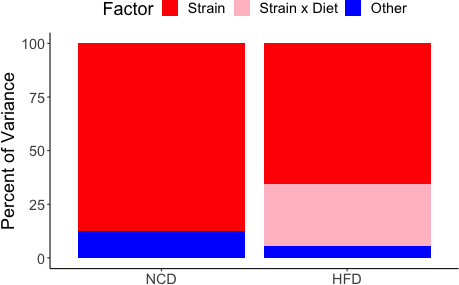
\includegraphics{figures/anova-barplots-1.png}

\begin{Shaded}
\begin{Highlighting}[]
\NormalTok{ee.var.all.data <-}\StringTok{ }\KeywordTok{bind_rows}\NormalTok{(lean.adj.ee.all }\OperatorTok\StringTok{ }\KeywordTok{mutate}\NormalTok{(}\DataTypeTok{Diet=}\StringTok{"NCD"}\NormalTok{,}\DataTypeTok{Corr=}\StringTok{"None"}\NormalTok{),}
\NormalTok{                             lean.adj.ee.lean }\OperatorTok\StringTok{ }\KeywordTok{mutate}\NormalTok{(}\DataTypeTok{Diet=}\StringTok{"NCD"}\NormalTok{, }\DataTypeTok{Corr=}\StringTok{"Lean Mass"}\NormalTok{),}
\NormalTok{                             hfd.adj.ee.all }\OperatorTok\StringTok{ }\KeywordTok{mutate}\NormalTok{(}\DataTypeTok{Diet=}\StringTok{"HFD"}\NormalTok{, }\DataTypeTok{Corr=}\StringTok{"Lean Mass"}\NormalTok{),}
\NormalTok{                             hfd.adj.ee.adj }\OperatorTok\StringTok{ }\KeywordTok{mutate}\NormalTok{(}\DataTypeTok{Diet=}\StringTok{"HFD"}\NormalTok{, }\DataTypeTok{Corr=}\StringTok{"Lean Mass,Diet"}\NormalTok{)) }\OperatorTok
\StringTok{  }\KeywordTok{mutate}\NormalTok{(}\DataTypeTok{Group=}\KeywordTok{paste}\NormalTok{(Diet,Corr,}\DataTypeTok{sep=}\StringTok{"-"}\NormalTok{))}

\KeywordTok{library}\NormalTok{(RColorBrewer)}
\NormalTok{ee.var.all.data }\OperatorTok\StringTok{ }
\StringTok{         }\KeywordTok{filter}\NormalTok{(term }\OperatorTok\StringTok{ }\KeywordTok{c}\NormalTok{(}\StringTok{'Lean'}\NormalTok{,}\StringTok{'Name'}\NormalTok{,}\StringTok{'Name:Diet'}\NormalTok{,}\StringTok{'Diet'}\NormalTok{,}\StringTok{'Residuals'}\NormalTok{)) }\OperatorTok
\StringTok{         }\KeywordTok{filter}\NormalTok{(}\OperatorTok{!}\NormalTok{(term}\OperatorTok{==}\StringTok{'Lean'}\OperatorTok{&}\NormalTok{Corr}\OperatorTok{==}\StringTok{'Lean Mass'}\NormalTok{)) }\OperatorTok
\StringTok{         }\KeywordTok{filter}\NormalTok{(}\OperatorTok{!}\NormalTok{(term}\OperatorTok{==}\StringTok{'Lean'}\OperatorTok{&}\NormalTok{Corr}\OperatorTok{==}\StringTok{"Lean Mass,Diet"}\NormalTok{)) }\OperatorTok
\StringTok{         }\KeywordTok{filter}\NormalTok{(}\OperatorTok{!}\NormalTok{(term}\OperatorTok{==}\StringTok{'Diet'}\OperatorTok{&}\NormalTok{Corr}\OperatorTok{==}\StringTok{"Lean Mass,Diet"}\NormalTok{)) }\OperatorTok
\KeywordTok{ggplot}\NormalTok{(}\KeywordTok{aes}\NormalTok{(}\DataTypeTok{x=}\KeywordTok{ordered}\NormalTok{(Group, }\DataTypeTok{levels=}\KeywordTok{c}\NormalTok{(}\StringTok{"NCD-None"}\NormalTok{,}\StringTok{"NCD-Lean Mass"}\NormalTok{, }\StringTok{"HFD-Lean Mass"}\NormalTok{, }\StringTok{"HFD-Lean Mass,Diet"}\NormalTok{)),}
            \DataTypeTok{y=}\NormalTok{Pct.Var,}
            \DataTypeTok{fill=}\NormalTok{term)) }\OperatorTok{+}
\StringTok{  }\KeywordTok{geom_bar}\NormalTok{(}\DataTypeTok{position=}\StringTok{"stack"}\NormalTok{,}\DataTypeTok{stat=}\StringTok{'identity'}\NormalTok{) }\OperatorTok{+}
\StringTok{  }\KeywordTok{scale_fill_manual}\NormalTok{(}\DataTypeTok{name=}\StringTok{"Factor"}\NormalTok{,}
                    \DataTypeTok{labels =} \KeywordTok{c}\NormalTok{(}\StringTok{"Diet"}\NormalTok{, }\StringTok{"Lean Mass"}\NormalTok{, }\StringTok{"Strain"}\NormalTok{, }\StringTok{"Strain x Diet"}\NormalTok{, }\StringTok{"Residuals"}\NormalTok{),}
                    \DataTypeTok{values=}\KeywordTok{brewer.pal}\NormalTok{(}\DecValTok{5}\NormalTok{, }\StringTok{"Set1"}\NormalTok{)) }\OperatorTok{+}
\StringTok{  }\KeywordTok{labs}\NormalTok{(}\DataTypeTok{y=}\StringTok{"Variance Contribution (%)"}\NormalTok{,}
       \DataTypeTok{x=}\StringTok{"Diet and Adjustments"}\NormalTok{) }\OperatorTok{+}
\StringTok{  }\KeywordTok{theme_classic}\NormalTok{() }\OperatorTok{+}
\StringTok{  }\KeywordTok{theme}\NormalTok{(}\DataTypeTok{text=}\KeywordTok{element_text}\NormalTok{(}\DataTypeTok{size=}\DecValTok{18}\NormalTok{),}
        \DataTypeTok{axis.text=}\KeywordTok{element_text}\NormalTok{(}\DataTypeTok{size=}\DecValTok{8}\NormalTok{))}
\end{Highlighting}
\end{Shaded}

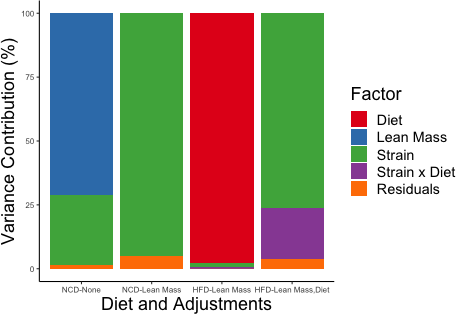
\includegraphics{figures/anova-barplots-2.png}

\hypertarget{adaptive-thermogenesis-vs-weight-gain}{%
\subsubsection{Adaptive Thermogenesis vs Weight
Gain}\label{adaptive-thermogenesis-vs-weight-gain}}

\begin{Shaded}
\begin{Highlighting}[]
\NormalTok{data.wide }\OperatorTok
\StringTok{  }\KeywordTok{ggplot}\NormalTok{(}\KeywordTok{aes}\NormalTok{(}\DataTypeTok{y=}\NormalTok{Wt.Gain,}
             \DataTypeTok{x=}\NormalTok{AT)) }\OperatorTok{+}
\StringTok{  }\KeywordTok{labs}\NormalTok{(}\DataTypeTok{y=}\StringTok{"Weight Gained on HFD (g)"}\NormalTok{,}
       \DataTypeTok{x=}\StringTok{"Adaptive Thermogenesis (W)"}\NormalTok{) }\OperatorTok{+}
\StringTok{  }\KeywordTok{geom_point}\NormalTok{() }\OperatorTok{+}
\StringTok{  }\KeywordTok{geom_smooth}\NormalTok{(}\DataTypeTok{method=}\StringTok{"lm"}\NormalTok{) }\OperatorTok{+}\StringTok{  }\KeywordTok{theme_classic}\NormalTok{() }\OperatorTok{+}
\StringTok{  }\KeywordTok{theme}\NormalTok{(}\DataTypeTok{text=}\KeywordTok{element_text}\NormalTok{(}\DataTypeTok{size=}\DecValTok{18}\NormalTok{))}
\end{Highlighting}
\end{Shaded}

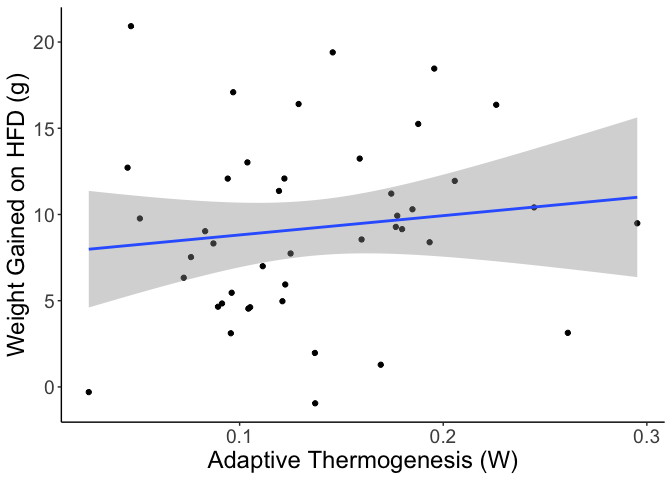
\includegraphics{figures/adaptive-thermogenesis-weight-1.png}

\begin{Shaded}
\begin{Highlighting}[]
\KeywordTok{lm}\NormalTok{(Wt.Gain}\OperatorTok{~}\NormalTok{AT, }\DataTypeTok{data=}\NormalTok{data.wide) }\OperatorTok\StringTok{ }\NormalTok{glance }\OperatorTok\StringTok{ }\KeywordTok{kable}\NormalTok{(}\DataTypeTok{caption=}\StringTok{"Summary of relationship between energy expenditure and diet-induced weight gain"}\NormalTok{)}
\end{Highlighting}
\end{Shaded}

\begin{longtable}[]{@{}rrrrrrrrrrrr@{}}
\caption{Summary of relationship between energy expenditure and
diet-induced weight gain}\tabularnewline
\toprule
\begin{minipage}[b]{0.08\columnwidth}\raggedleft
r.squared\strut
\end{minipage} & \begin{minipage}[b]{0.11\columnwidth}\raggedleft
adj.r.squared\strut
\end{minipage} & \begin{minipage}[b]{0.05\columnwidth}\raggedleft
sigma\strut
\end{minipage} & \begin{minipage}[b]{0.08\columnwidth}\raggedleft
statistic\strut
\end{minipage} & \begin{minipage}[b]{0.06\columnwidth}\raggedleft
p.value\strut
\end{minipage} & \begin{minipage}[b]{0.02\columnwidth}\raggedleft
df\strut
\end{minipage} & \begin{minipage}[b]{0.05\columnwidth}\raggedleft
logLik\strut
\end{minipage} & \begin{minipage}[b]{0.03\columnwidth}\raggedleft
AIC\strut
\end{minipage} & \begin{minipage}[b]{0.03\columnwidth}\raggedleft
BIC\strut
\end{minipage} & \begin{minipage}[b]{0.07\columnwidth}\raggedleft
deviance\strut
\end{minipage} & \begin{minipage}[b]{0.09\columnwidth}\raggedleft
df.residual\strut
\end{minipage} & \begin{minipage}[b]{0.04\columnwidth}\raggedleft
nobs\strut
\end{minipage}\tabularnewline
\midrule
\endfirsthead
\toprule
\begin{minipage}[b]{0.08\columnwidth}\raggedleft
r.squared\strut
\end{minipage} & \begin{minipage}[b]{0.11\columnwidth}\raggedleft
adj.r.squared\strut
\end{minipage} & \begin{minipage}[b]{0.05\columnwidth}\raggedleft
sigma\strut
\end{minipage} & \begin{minipage}[b]{0.08\columnwidth}\raggedleft
statistic\strut
\end{minipage} & \begin{minipage}[b]{0.06\columnwidth}\raggedleft
p.value\strut
\end{minipage} & \begin{minipage}[b]{0.02\columnwidth}\raggedleft
df\strut
\end{minipage} & \begin{minipage}[b]{0.05\columnwidth}\raggedleft
logLik\strut
\end{minipage} & \begin{minipage}[b]{0.03\columnwidth}\raggedleft
AIC\strut
\end{minipage} & \begin{minipage}[b]{0.03\columnwidth}\raggedleft
BIC\strut
\end{minipage} & \begin{minipage}[b]{0.07\columnwidth}\raggedleft
deviance\strut
\end{minipage} & \begin{minipage}[b]{0.09\columnwidth}\raggedleft
df.residual\strut
\end{minipage} & \begin{minipage}[b]{0.04\columnwidth}\raggedleft
nobs\strut
\end{minipage}\tabularnewline
\midrule
\endhead
\begin{minipage}[t]{0.08\columnwidth}\raggedleft
0.017\strut
\end{minipage} & \begin{minipage}[t]{0.11\columnwidth}\raggedleft
-0.007\strut
\end{minipage} & \begin{minipage}[t]{0.05\columnwidth}\raggedleft
5.22\strut
\end{minipage} & \begin{minipage}[t]{0.08\columnwidth}\raggedleft
0.691\strut
\end{minipage} & \begin{minipage}[t]{0.06\columnwidth}\raggedleft
0.411\strut
\end{minipage} & \begin{minipage}[t]{0.02\columnwidth}\raggedleft
1\strut
\end{minipage} & \begin{minipage}[t]{0.05\columnwidth}\raggedleft
-131\strut
\end{minipage} & \begin{minipage}[t]{0.03\columnwidth}\raggedleft
268\strut
\end{minipage} & \begin{minipage}[t]{0.03\columnwidth}\raggedleft
273\strut
\end{minipage} & \begin{minipage}[t]{0.07\columnwidth}\raggedleft
1117\strut
\end{minipage} & \begin{minipage}[t]{0.09\columnwidth}\raggedleft
41\strut
\end{minipage} & \begin{minipage}[t]{0.04\columnwidth}\raggedleft
43\strut
\end{minipage}\tabularnewline
\bottomrule
\end{longtable}

\hypertarget{integration-with-lifespan}{%
\section{Integration with Lifespan}\label{integration-with-lifespan}}

To ask whether BMR is related to experimental livespan we used the data
from Roy et al 2021. This determined lifespan of \textbf{female} mice in
days

\begin{Shaded}
\begin{Highlighting}[]
\NormalTok{aging.datafile <-}\StringTok{ 'BXD_18441.csv'}

\NormalTok{aging.data <-}\StringTok{ }\KeywordTok{read_csv}\NormalTok{(aging.datafile, }\DataTypeTok{skip=}\DecValTok{8}\NormalTok{) }\OperatorTok
\StringTok{  }\KeywordTok{rename}\NormalTok{(}\DataTypeTok{Age =}\NormalTok{ Value,}
         \DataTypeTok{Age.SE =}\NormalTok{ SE,}
         \DataTypeTok{Age.N =}\NormalTok{ N)}

\NormalTok{combined.age.mr.data <-}
\StringTok{  }\KeywordTok{full_join}\NormalTok{(aging.data, data.wide)}

\NormalTok{combined.age.mr.data }\OperatorTok
\StringTok{  }\KeywordTok{ggplot}\NormalTok{(}\KeywordTok{aes}\NormalTok{(}\DataTypeTok{y=}\NormalTok{Age,}
             \DataTypeTok{x=}\NormalTok{MR_adj_NCD)) }\OperatorTok{+}
\StringTok{  }\KeywordTok{geom_point}\NormalTok{() }\OperatorTok{+}
\StringTok{  }\KeywordTok{geom_errorbar}\NormalTok{(}\KeywordTok{aes}\NormalTok{(}\DataTypeTok{ymin=}\NormalTok{Age}\OperatorTok{-}\NormalTok{Age.SE,}
                    \DataTypeTok{ymax=}\NormalTok{Age}\OperatorTok{+}\NormalTok{Age.SE),}
                \DataTypeTok{alpha=}\FloatTok{0.25}\NormalTok{) }\OperatorTok{+}
\StringTok{  }\KeywordTok{geom_errorbarh}\NormalTok{(}\KeywordTok{aes}\NormalTok{(}\DataTypeTok{xmin=}\NormalTok{MR_adj_NCD}\OperatorTok{-}\NormalTok{MR_W_SE_NCD,}
                    \DataTypeTok{xmax=}\NormalTok{MR_adj_NCD}\OperatorTok{+}\NormalTok{MR_W_SE_NCD),}
                \DataTypeTok{alpha=}\FloatTok{0.25}\NormalTok{) }\OperatorTok{+}
\StringTok{  }\KeywordTok{geom_smooth}\NormalTok{(}\DataTypeTok{method=}\StringTok{"lm"}\NormalTok{) }\OperatorTok{+}
\StringTok{  }\KeywordTok{theme_classic}\NormalTok{() }\OperatorTok{+}
\StringTok{  }\KeywordTok{theme}\NormalTok{(}\DataTypeTok{text=}\KeywordTok{element_text}\NormalTok{(}\DataTypeTok{size=}\DecValTok{18}\NormalTok{))}
\end{Highlighting}
\end{Shaded}

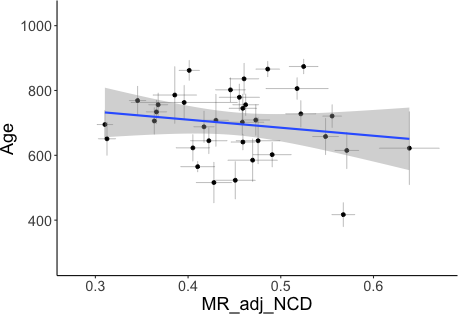
\includegraphics{figures/aging-data-1.png}

\begin{Shaded}
\begin{Highlighting}[]
\NormalTok{combined.age.mr.data }\OperatorTok
\StringTok{  }\KeywordTok{mutate_at}\NormalTok{(}\KeywordTok{vars}\NormalTok{(Age,MR_adj_NCD), }\DataTypeTok{.funs=}\NormalTok{as.numeric) }\OperatorTok
\StringTok{  }\KeywordTok{summarize_at}\NormalTok{(}\KeywordTok{vars}\NormalTok{(Age,MR_adj_NCD), }\DataTypeTok{.funs=}\ControlFlowTok{function}\NormalTok{(x) }\KeywordTok{shapiro.test}\NormalTok{(x)}\OperatorTok{$}\NormalTok{p.value) }\OperatorTok
\StringTok{  }\KeywordTok{kable}\NormalTok{(}\DataTypeTok{caption=}\StringTok{"Shapiro-Wilk tests for normality"}\NormalTok{)}
\end{Highlighting}
\end{Shaded}

\begin{longtable}[]{@{}rr@{}}
\caption{Shapiro-Wilk tests for normality}\tabularnewline
\toprule
Age & MR\_adj\_NCD\tabularnewline
\midrule
\endfirsthead
\toprule
Age & MR\_adj\_NCD\tabularnewline
\midrule
\endhead
0.98 & 0.043\tabularnewline
\bottomrule
\end{longtable}

\begin{Shaded}
\begin{Highlighting}[]
\KeywordTok{with}\NormalTok{(combined.age.mr.data, }\KeywordTok{cor.test}\NormalTok{(Age, MR_adj_NCD)) }\OperatorTok\StringTok{ }
\StringTok{  }\NormalTok{tidy }\OperatorTok
\StringTok{  }\KeywordTok{kable}\NormalTok{(}\DataTypeTok{caption=}\StringTok{"Relationship between age (of female BXD mice) and adjusted metabolic rate"}\NormalTok{)}
\end{Highlighting}
\end{Shaded}

\begin{longtable}[]{@{}rrrrrrll@{}}
\caption{Relationship between age (of female BXD mice) and adjusted
metabolic rate}\tabularnewline
\toprule
\begin{minipage}[b]{0.07\columnwidth}\raggedleft
estimate\strut
\end{minipage} & \begin{minipage}[b]{0.07\columnwidth}\raggedleft
statistic\strut
\end{minipage} & \begin{minipage}[b]{0.06\columnwidth}\raggedleft
p.value\strut
\end{minipage} & \begin{minipage}[b]{0.07\columnwidth}\raggedleft
parameter\strut
\end{minipage} & \begin{minipage}[b]{0.07\columnwidth}\raggedleft
conf.low\strut
\end{minipage} & \begin{minipage}[b]{0.07\columnwidth}\raggedleft
conf.high\strut
\end{minipage} & \begin{minipage}[b]{0.28\columnwidth}\raggedright
method\strut
\end{minipage} & \begin{minipage}[b]{0.09\columnwidth}\raggedright
alternative\strut
\end{minipage}\tabularnewline
\midrule
\endfirsthead
\toprule
\begin{minipage}[b]{0.07\columnwidth}\raggedleft
estimate\strut
\end{minipage} & \begin{minipage}[b]{0.07\columnwidth}\raggedleft
statistic\strut
\end{minipage} & \begin{minipage}[b]{0.06\columnwidth}\raggedleft
p.value\strut
\end{minipage} & \begin{minipage}[b]{0.07\columnwidth}\raggedleft
parameter\strut
\end{minipage} & \begin{minipage}[b]{0.07\columnwidth}\raggedleft
conf.low\strut
\end{minipage} & \begin{minipage}[b]{0.07\columnwidth}\raggedleft
conf.high\strut
\end{minipage} & \begin{minipage}[b]{0.28\columnwidth}\raggedright
method\strut
\end{minipage} & \begin{minipage}[b]{0.09\columnwidth}\raggedright
alternative\strut
\end{minipage}\tabularnewline
\midrule
\endhead
\begin{minipage}[t]{0.07\columnwidth}\raggedleft
-0.058\strut
\end{minipage} & \begin{minipage}[t]{0.07\columnwidth}\raggedleft
-0.356\strut
\end{minipage} & \begin{minipage}[t]{0.06\columnwidth}\raggedleft
0.724\strut
\end{minipage} & \begin{minipage}[t]{0.07\columnwidth}\raggedleft
37\strut
\end{minipage} & \begin{minipage}[t]{0.07\columnwidth}\raggedleft
-0.367\strut
\end{minipage} & \begin{minipage}[t]{0.07\columnwidth}\raggedleft
0.262\strut
\end{minipage} & \begin{minipage}[t]{0.28\columnwidth}\raggedright
Pearson's product-moment correlation\strut
\end{minipage} & \begin{minipage}[t]{0.09\columnwidth}\raggedright
two.sided\strut
\end{minipage}\tabularnewline
\bottomrule
\end{longtable}

\hypertarget{session-information}{%
\section{Session Information}\label{session-information}}

\begin{Shaded}
\begin{Highlighting}[]
\KeywordTok{sessionInfo}\NormalTok{()}
\end{Highlighting}
\end{Shaded}

\begin{verbatim}
## R version 4.0.2 (2020-06-22)
## Platform: x86_64-apple-darwin17.0 (64-bit)
## Running under: macOS  10.16
## 
## Matrix products: default
## BLAS:   /Library/Frameworks/R.framework/Versions/4.0/Resources/lib/libRblas.dylib
## LAPACK: /Library/Frameworks/R.framework/Versions/4.0/Resources/lib/libRlapack.dylib
## 
## locale:
## [1] en_US.UTF-8/en_US.UTF-8/en_US.UTF-8/C/en_US.UTF-8/en_US.UTF-8
## 
## attached base packages:
## [1] stats     graphics  grDevices utils     datasets  methods   base     
## 
## other attached packages:
## [1] RColorBrewer_1.1-2 broom_0.7.11       ggrepel_0.9.1      ggplot2_3.3.5     
## [5] readr_2.1.1        dplyr_1.0.7        tidyr_1.1.4        knitr_1.37        
## 
## loaded via a namespace (and not attached):
##  [1] tidyselect_1.1.1 xfun_0.29        purrr_0.3.4      splines_4.0.2   
##  [5] lattice_0.20-45  colorspace_2.0-2 vctrs_0.3.8      generics_0.1.1  
##  [9] htmltools_0.5.2  yaml_2.2.1       mgcv_1.8-38      utf8_1.2.2      
## [13] rlang_0.4.12     pillar_1.6.4     glue_1.6.0       withr_2.4.3     
## [17] DBI_1.1.2        bit64_4.0.5      lifecycle_1.0.1  stringr_1.4.0   
## [21] munsell_0.5.0    gtable_0.3.0     evaluate_0.14    labeling_0.4.2  
## [25] tzdb_0.2.0       fastmap_1.1.0    parallel_4.0.2   fansi_1.0.0     
## [29] highr_0.9        Rcpp_1.0.7       backports_1.4.1  scales_1.1.1    
## [33] vroom_1.5.7      magick_2.7.3     farver_2.1.0     bit_4.0.4       
## [37] hms_1.1.1        digest_0.6.29    stringi_1.7.6    grid_4.0.2      
## [41] cli_3.1.0        tools_4.0.2      magrittr_2.0.1   tibble_3.1.6    
## [45] crayon_1.4.2     pkgconfig_2.0.3  ellipsis_0.3.2   Matrix_1.4-0    
## [49] assertthat_0.2.1 rmarkdown_2.11   rstudioapi_0.13  R6_2.5.1        
## [53] nlme_3.1-153     compiler_4.0.2
\end{verbatim}

\end{document}
